\documentclass[11pt,a4paper]{article}
\usepackage{fontspec}
\setmainfont{TeX Gyre Pagella}
\newfontfamily\headfont{Inter}[UprightFont=*-ExtraBold,BoldFont=*-ExtraBold,Extension=.otf,Path=/usr/share/fonts/opentype/inter/]
\usepackage[a4paper,margin=2.3cm]{geometry}
\usepackage{amsmath}
\usepackage{graphicx,booktabs,float,caption,array,xcolor,longtable,threeparttable}
\usepackage{xurl}
\usepackage[hidelinks]{hyperref}
\usepackage{titlesec}
\usepackage[round]{natbib}
\usepackage{setspace}
\setstretch{1.05}
\renewcommand{\topfraction}{0.9}
\renewcommand{\bottomfraction}{0.8}
\renewcommand{\textfraction}{0.1}
\renewcommand{\floatpagefraction}{0.75}
\setlength{\parindent}{0pt}
\setlength{\parskip}{0.55em}
\titleformat{\section}{\headfont\Large}{\thesection}{0.8em}{}
\titleformat{\subsection}{\headfont\large}{\thesubsection}{0.8em}{}
\captionsetup{font=small,labelfont=bf}
\urlstyle{same}
\hypersetup{pdftitle={The Half-Life of Fame},pdfauthor={Dr Tristan Hotham}}

\begin{document}
\begin{center}
{\Large\bfseries The Half-Life of Fame: How Attention to Notable People on English Wikipedia Rises and Decays after Their Deaths\par}
\vspace{1.2em}
{\large Dr Tristan Hotham\par}
\vspace{0.3em}
{\small Independent researcher\\
ORCID: 0000-0003-4931-9349\\
DOI: https://doi.org/10.5281/zenodo.24095452\par}
\vspace{0.8em}
2026
\end{center}

\begin{quote}
\small
\begin{center}\textbf{Abstract}\end{center}
Attention to notable people rises sharply when they die and then fades, but how far it fades, and for whom, has rarely been measured at scale. I follow the English Wikipedia articles of 16,397 people who died between 2016 and 2023 (a 30\% hash sample of Wikidata), measuring monthly user pageviews (looking someone up, not remembering them) as a share of all English Wikipedia traffic relative to each person's own level in the year before death. In an analysis pre-specified in a written plan, the median peak is 16.5 times the pre-death level. The decay is best described by two phases, with half-lives of about 11 days and 6.9 months, although a power law predicts later cohorts slightly better. Two to three years after death, the median person receives 0.98 (95\% CI 0.97 to 0.99) of their pre-death share; an exploratory comparison with the drift before death places this about 5\% above a no-death path. Age at death is the strongest correlate: people who died under 50 retain 63\% more long-run attention than those who died at 65 to 79 (95\% CI 51 to 77), a gap absent at a placebo date and present in all 21 robustness checks. Performers are the only occupational group whose typical attention settles above its baseline, but placebo tests show that the occupational gaps partly predate the deaths. Estimates for women and for citizens of English-speaking countries depend on specification and are not robust. The design is descriptive and observational.

\textbf{Keywords:} collective memory; attention decay; Wikipedia pageviews; death; fame; forgetting curves; Wikidata
\end{quote}

\section{Introduction}
The death of a well-known person is one of the most reliable triggers of collective attention. News organisations publish obituaries prepared in advance, friends and colleagues share memories, and large numbers of people turn to reference works to learn or relearn who the person was. On English Wikipedia these surges are among the largest in the encyclopedia's traffic: in the sample studied here, the article on the musician Prince received 17,545,455 user views in the month he died. The surges are brief. What happens afterwards is less visible and less studied: whether attention falls back to where it was, settles at a higher level because the death has made the person more salient, or drops below the old level because the public career that kept the person in view has ended.

This question touches several literatures. Studies of collective memory, from \citet{halbwachs1992} to the distinction between communicative and cultural memory drawn by \citet{assmann1995}, describe how a society's memory of people and events is carried first by living conversation and then by institutions and records. Quantitative work has begun to measure the timing of this transition: \citet{candia2019} show that attention to cultural products, including biographies, decays according to a biexponential function, which they interpret as the sum of a fast communicative component and a slow cultural one. Work on online attention has found power-law and stretched-exponential relaxations after bursts \citep{wu2007,crane2008,ratkiewicz2010,lehmann2012}. Psychological research on individual forgetting has long debated whether forgetting curves are exponential or power functions \citep{wixted1991,rubin1996}, and \citet{roediger2014} extend the forgetting curve to the collective memory of United States presidents.

Deaths are a distinctive event within this landscape because they are both a moment of maximal attention and an end to new achievements. \citet{keegan2015} show how Wikipedia editors coordinate to update biographies in the hours after a death, and \citet{west2021} track mentions of 2,362 public figures in news and on Twitter for a year either side of their deaths, finding a sharp spike and rapid decay, with larger long-term boosts for artists and for those who died young or unnaturally. Studies of the art market describe a ``death effect'' on prices \citep{ekelund2000}, and historical work on artistic reputations finds that most artists' reputations peak around death and then decline \citep{zhang2023}.

This paper contributes a large-scale, pre-specified measurement of the post-mortem attention curve on the world's most used reference work, with three features that earlier work lacks. First, each person's attention is normalised by their own pre-death level, so that the curve measures change rather than fame, and by the total traffic of English Wikipedia, which declined over the period. Second, the sample is a fixed pseudo-random draw from every person with an English Wikipedia article who died in 2016 to 2023 according to Wikidata, not a list of celebrities, so it includes the many modestly notable people who make up most of the encyclopedia's biographies. Third, the analysis plan, including the decay models compared, the long-run window and the regression specification, was written before any post-death outcome was computed (it is reproduced in the replication materials), and the paper reports the planned specifications as the main results, including those that disappoint.

The answers are, in brief, these. The median peak is 16.5 times the pre-death level. The decay has a fast phase with a half-life of about 11 days and a slow phase with a half-life of about 6.9 months. Two to three years after death the median person is back to 0.98 of their earlier share of attention, slightly below it, with 47.8\% above. A death does not, for the typical person, leave a lasting increase in attention, although it may slow a decline that was already under way. Age at death is the clearest correlate of lasting attention, and it survives a placebo test that the occupational differences only partly survive.

The rest of the paper reviews the relevant work (Section~\ref{sec:lit}), describes the data (Section~\ref{sec:data}) and design (Section~\ref{sec:design}), reports results (Section~\ref{sec:results}) and robustness (Section~\ref{sec:robust}), and discusses limitations (Section~\ref{sec:disc}).

\section{Background and literature}\label{sec:lit}
\subsection{Collective memory and its decay}
\citet{halbwachs1992} argued that memory is social: individuals remember within frameworks supplied by the groups they belong to. Later work distinguished between the memory carried by living people in everyday communication and the memory fixed in texts, monuments and institutions. \citet{assmann1995} called these communicative and cultural memory, and placed the horizon of communicative memory at around three generations. \citet{olick1998} review how sociologists turned these ideas into a historical sociology of mnemonic practices. The present paper does not measure memory in this rich sense; it measures one observable practice, looking someone up in an encyclopedia, and treats its time course as an indicator of how quickly a person passes from the news into the record.

The quantitative turn in this area owes much to digitised text and online traces. \citet{michel2011} used millions of digitised books to show how the fame of people born in different periods rose and fell, and how quickly mentions of past years faded from print. \citet{skiena2013} ranked historical figures by combining Wikipedia page length, edits and page traffic with other signals. \citet{roediger2014} measured how successive cohorts of Americans forget past presidents, and fitted forgetting curves to predict when recent presidents will fade. \citet{candia2019} brought these strands together in a model of collective memory in which attention to cultural products, including papers, patents, songs, films and biographies, decays as the sum of two exponentials: a fast-decaying communicative memory and a slower cultural memory. They found that this biexponential function fits better than exponential and log-normal alternatives, and that biographies remain in communicative memory longest. The present paper borrows this model but applies it to a sharper event, a death, and to a much shorter horizon, months rather than decades.

\subsection{Attention dynamics online}
A separate line of work in physics and computer science has modelled how online attention responds to shocks. \citet{wu2007} found that the novelty of stories on a social news site decays, in aggregate, as a stretched exponential. \citet{crane2008} classified bursts of YouTube views by their relaxation after a peak, finding power-law decays whose exponents distinguish exogenous from endogenous shocks. \citet{ratkiewicz2010} found that Wikipedia and web popularity arrive in bursts with heavy-tailed sizes, and \citet{lehmann2012} identified classes of hashtag attention on Twitter by the share of activity before, during and after the peak. These studies suggest two expectations for the post-mortem curve: a sharply peaked exogenous shock should relax quickly, and the long-run tail may follow a power law rather than an exponential. Psychology offers a parallel debate. \citet{wixted1991} found that power functions describe individual forgetting better than exponentials, and \citet{rubin1996}, fitting 105 functions to 210 retention data sets, found that several two-parameter forms fit about equally well. Distinguishing exponential, power-law and two-phase decay is therefore not only a question of fit statistics but of which model generalises, which is why the plan below includes an out-of-sample comparison.

Wikipedia pageviews have become a standard measure of public attention. They have been used to forecast box office revenue \citep{mestyan2013} and to describe why readers come to the encyclopedia \citep{singer2017}, including how readers outside the English-speaking world use it \citep{lemmerich2019}. \citet{garciagavilanes2017} used pageviews of articles on aviation accidents to show how a new disaster triggers renewed attention to past ones, and \citet{kanhabua2014} identified which kinds of events trigger remembering of older events on Wikipedia. These studies treat pageviews as an indicator of what the public is curious about at a given moment; that is the sense in which they are used here.

\subsection{Death, commemoration and attention}
\citet{keegan2015} studied the editing of Wikipedia biographies after their subjects died, showing how editors coordinate on changes of tense and on commemoration, and how the articles become sites of collective mourning. Their focus was on editors; the present paper turns to readers. The closest study is by \citet{west2021}, who followed 2,362 public figures through English-language news and Twitter for a year before and after death. They found a spike followed by a rapid decay, modelled the curve with communicative and cultural components, and reported that the largest boosts went to popular anglophones who died young or unnaturally, and that long-term boosts were smallest for leaders and largest for artists. The present study differs in its source (an encyclopedia rather than news), its sample (all people with an English Wikipedia article who died in the period, in a pseudo-random sample, rather than people prominent enough to be tracked in the news), its horizon (up to five years) and its normalisation (each person's own pre-death attention). A popular data essay on Wikipedia traffic after celebrity deaths \citep{samora2018} illustrated the size of the spikes for the best-known cases.

Economists have studied whether deaths raise the value of an artist's work. \citet{ekelund2000} found that artists' auction prices rise around the time of death and discussed demand-side explanations. \citet{zhang2023} tracked the reputations of over 3,300 artists from 1795 to 2020 in a large corpus and found that most peak just before death and then decline, including those who died young or unexpectedly. These findings raise the question of whether online attention, too, peaks at death and then falls below its earlier level.

\subsection{Who is remembered}
A large literature documents inequalities in who is recorded and remembered. Wikipedia's coverage of women is lower than of men, and women's biographies differ in content and linking \citep{wagner2015,graellsgarrido2015,wagner2016}. \citet{wagner2016} report that women in Wikipedia are on average more notable than men, which they interpret as a glass ceiling: the bar for inclusion is higher. \citet{konieczny2018} track the gender gap across time and cultures using Wikidata. Databases of notable people built from Wikipedia and Wikidata \citep{yu2016,gergaud2016,laouenan2022} show how coverage varies by period, place, language and occupation, and \citet{laouenan2022} document an Anglo-Saxon bias in English-language sources. The Matthew effect \citep{merton1968} suggests that attention accrues to those who already have it; \citet{zhang2023} find the opposite for artistic reputations after death. These literatures motivate the comparisons by occupation, sex, citizenship and prior fame below.

\subsection{What is new here}
The contribution is a pre-specified, large-scale and normalised measurement of the post-mortem attention curve, including its long-run settling point relative to each person's own baseline, for a pseudo-random sample of the people English Wikipedia covers. It adds a placebo design that separates the effect of the death from the trends attention was already following, and it reports how much of the variation by age, occupation, sex and citizenship survives that separation. It also documents a group that most studies cannot see: people whose English Wikipedia article was first read only when they died.

\section{Data}\label{sec:data}
\subsection{People}
The population is every Wikidata item that is an instance of human, has an English Wikipedia article, and has a date of death from 2016 to 2023, retrieved through QLever with the article title, date of birth, sex, one sampled occupation, one sampled country of citizenship and the number of Wikipedia language editions (sitelinks) \citep{vrandecic2014}. The query returned 100,689 rows for 98,246 people; rows repeat where an item has more than one date of birth or death. I kept the earliest date of death and the earliest date of birth, set age to missing where two dates of birth differ by more than a year (400 people), and kept the first occupation whose broad family is not ``other''. Dates of death on 1 January (9,334 people) may be year-precision values, since the export does not carry date precision, and are excluded from the main sample by a rule set in advance.

Occupations were grouped into ten families by keyword rules on the English label of the occupation and of its superclass, with a short list of manual overrides for labels the rules misclassify (for example, ``political scientist'' is academic, not political). The full table of 2,557 occupation labels and their families is released with the data. The families are performers (actors, musicians, singers, directors and other film and stage professions), writers and artists, sport, politics and law, science and academia, business, the military, religion, journalism and media, and other. Wikidata gives several occupations for many people; only one was sampled by the query, so families describe one of possibly several roles. Citizenship was coded as English-speaking (United States, United Kingdom, Canada, Australia, New Zealand, Ireland), other, or unknown.

\subsection{Pageviews}
For a fixed 30\% sample of these people, defined by a hash of the Wikidata identifier ($h \leftarrow 31h + c \bmod 2^{32}$ over the characters $c$ of the identifier, keeping $h \bmod 10 < 3$), monthly English Wikipedia pageviews by the agent type ``user'' were retrieved from the Wikimedia pageviews interface for July 2015 (the first month available) to October 2026. The ``user'' agent excludes self-identified crawlers and traffic flagged as automated by Wikimedia's heuristics. The hash reproduces the sample exactly (29,384 people). Of these, 29,364 were fetched, 9 returned no article under the stored title (renamed or deleted pages) and 20 fetches failed. Months with no views are absent from the interface's response and were set to zero between a series' first and last months. Total monthly English Wikipedia user views for the same period were retrieved for normalisation; they fell by 20\% between July 2015 and October 2026.

\subsection{Sample}
Table~\ref{tab:flow} shows the path from the sample to the analysis sample. The main restriction is that a person's article must have existed, in the sense of having received views under its current title, by the start of the baseline year. 9,421 people fail this test. Most of them (8,650) were first read in or after the month of death. Of those, 4,126 were first read in the month of death or the month after, which I interpret as articles created upon the death, and 4,524 were first read two or more months after the death; the latter are either articles moved to a new title after the death (for example to add a disambiguating phrase), whose earlier views are recorded under the old title, or articles written months or years after the death (median 28 months); the pageview data cannot separate the two. These people are analysed separately in Section~\ref{sec:posthumous}. People who died before February 2016 have fewer than six baseline months in the data and are excluded, as are 418 with no views at all in the baseline months.

\begin{table}[tbp]\centering\small\caption{From the Wikidata population to the analysis sample.}\label{tab:flow}\begin{tabular}{lr}\toprule Step & People\\\midrule
English Wikipedia articles, died 2016 to 2023 (Wikidata) & 98,246\\
30\% hash sample & 29,384\\
\quad with monthly pageviews (fetched, article found) & 29,355\\
\quad less: date of death on 1 January (possible year precision) & $-$2,827\\
\quad less: died before February 2016 (under six baseline months) & $-$292\\
\quad less: article not yet read at the start of the baseline & $-$9,421\\
\qquad of which first read in or after the month of death & 8,650\\
\quad less: no views in the baseline months & $-$418\\\midrule
Main sample & 16,397\\\bottomrule\end{tabular}\end{table}

The hash sample is representative of the full population on the observable characteristics: women make up 17.9\% of the full population and 17.7\% of the sample, the median number of sitelinks is 3 in both, and the shares of each occupation family differ by at most half a percentage point (Appendix Table~\ref{tab:rep}). The main sample differs from the population in predictable ways: it excludes people whose articles were created on their death, who are less often sportspeople and have fewer sitelinks, and those whose current title was first read two or more months after the death, who are more often women (24.6\% against 15.0\%) and less often citizens of English-speaking countries (27.9\% against 50.0\%), with a median of 2 sitelinks against 5 (exploratory comparison). Estimates for women and for citizenship therefore refer to people whose articles existed, under their current title, before their deaths.

\subsection{Measures}
For person $i$ who died in calendar month $d_i$, let $v_{it}$ be user views in month $t$ and $V_t$ total English Wikipedia user views. The attention share is $s_{it} = v_{it} / V_t$ and event time is $k = t - d_i$, so that $k = 0$ is the month of death. Because the month of death contains days before the death, the peak is defined over $k = 0$ and $k = 1$. The baseline is the mean share over $k = -12$ to $-2$; $k = -1$ is excluded because illness or news before a death can raise attention. The main measures are ratios to this baseline:
\begin{itemize}
\item Peak: $\max(s_{i0}, s_{i1}) / \bar s_i^{\,base}$.
\item One-year ratio: mean share over $k = 10$ to $14$, divided by the baseline.
\item Long-run ratio (LR): mean share over $k = 24$ to $34$, divided by the baseline. The data end in October 2026, so 34 months is the longest window every death in the sample can observe; the planning brief suggested 24 to 36.
\end{itemize}
Ratios are analysed on the log scale, with a floor of 0.05 before taking logs. Aggregate curves are the medians of $R_{ik} = s_{ik} / \bar s_i^{\,base}$ across people for each $k$, with 95\% intervals from 500 bootstrap resamples of people. Because a single month varies around the mean of its year, the median single-month ratio before death is about 0.95 rather than 1, while the window-averaged LR is directly comparable with its baseline.

The main sample comprises 16,397 people. Women are 15.0\%, citizens of English-speaking countries 50.0\% and the median age at death is 82.8. Table~\ref{tab:desc} describes the main measures by occupation family.

\begin{table}[tbp]\centering\small\caption{Medians by occupation family: peak, one-year ratio and long-run ratio (LR, with 95\% bootstrap interval), share of people with LR above 1, and the half-lives of the fast (days) and slow (months) components of a two-phase model fitted to each family's median curve (point estimates).}\label{tab:desc}\setlength{\tabcolsep}{4pt}\begin{tabular}{lrrrlrrr}\toprule Family & $N$ & Peak & Year 1 & LR & LR$>$1 (\%) & Fast (d) & Slow (mo)\\\midrule
Performers & 2,648 & 18.2 & 1.17 & 1.10 [1.09, 1.12] & 60 & 10 & 4.4\\
Sport & 4,306 & 23.1 & 1.08 & 0.99 [0.98, 1.01] & 50 & 10 & 5.3\\
Writers and artists & 1,961 & 13.3 & 1.08 & 0.99 [0.97, 1.01] & 48 & 12 & 8.7\\
Journalism and media & 536 & 26.0 & 1.06 & 0.95 [0.91, 0.99] & 45 & 13 & 11.7\\
Politics and law & 2,741 & 18.2 & 1.00 & 0.93 [0.90, 0.94] & 43 & 10 & 6.1\\
Science and academia & 2,412 & 9.7 & 1.03 & 0.93 [0.91, 0.94] & 42 & 14 & 12.1\\
Other & 630 & 9.8 & 0.99 & 0.92 [0.86, 0.97] & 43 & 13 & 9.2\\
Business & 499 & 14.7 & 0.99 & 0.92 [0.89, 0.95] & 42 & 14 & 8.7\\
Military & 302 & 10.0 & 1.00 & 0.92 [0.84, 0.97] & 42 & 14 & 16.2\\
Religion & 362 & 20.1 & 0.93 & 0.83 [0.79, 0.89] & 34 & 12 & 9.4\\
\midrule All & 16,397 & 16.5 & 1.06 & 0.98 [0.97, 0.99] & 48 & 11 & 6.9\\
\bottomrule\end{tabular}\end{table}

\section{Research design}\label{sec:design}
\subsection{Analysis plan}
The plan was written in the project notes after the data construction and before any post-death outcome was computed. It specified the measures above, the decay models, the hypotheses and what would count against them, the main regression and the robustness checks. Four changes were made after the first run, none after reading a regression coefficient: occupation keyword rules matched inside words (``rector'' inside ``director'') and were changed to match at word starts; the planned half-life of the excess remaining at $k = 1$ turned out to be under a month and is reported alongside the two component half-lives of the preferred model; and two exploratory checks were added and are labelled as such: a second placebo date 36 months before death, and the main models without the baseline control.

\subsection{Decay models}
Three models were fitted by least squares on the log of the median curve for $k = 1$ to 60:
\begin{align*}
\text{exponential:}\quad & R_k = c + a\,e^{-k/\tau},\\
\text{power law:}\quad & R_k = c + a\,k^{-b},\\
\text{two-phase:}\quad & R_k = c + a\,e^{-k/\tau_1} + b\,e^{-k/\tau_2},
\end{align*}
where $c$ is the level at which attention settles. The two-phase model is the biexponential of \citet{candia2019}. Models were compared by the Akaike information criterion on the log residuals and, to guard against overfitting, by the out-of-sample error when fitted to the median curve of deaths in 2016 to 2019 and used to predict that of deaths in 2020 to 2023 ($k = 1$ to 34). The pre-set criterion was that the two-phase model should win on both. Half-lives of the components are $\tau \ln 2$.

\subsection{Regression}
To ask who keeps attention, I estimate
\begin{equation*}
\log Y_i = \alpha + \textstyle\sum_f \beta_f F_{if} + \gamma\,\text{Woman}_i + \textstyle\sum_a \delta_a A_{ia} + \lambda\,\text{English}_i + \mu \log L_i + \rho \log \bar s_i^{\,base} + \eta_{y(i)} + \theta_{m(i)} + \varepsilon_i,
\end{equation*}
where $Y_i$ is LR (the main outcome), the peak or the one-year ratio; $F$ are occupation family indicators (reference: performers); $A$ are age-at-death bands (under 50, 50 to 64, 80 to 89, 90 and over; reference 65 to 79; unknown age as its own band); English is English-speaking citizenship (with unknown citizenship as its own category); $L$ is the number of sitelinks, a proxy for international fame before death; the log baseline share controls for the level of attention before death; and $\eta$ and $\theta$ are year and calendar-month-of-death fixed effects. Standard errors are clustered by month of death (95 clusters; estimation in statsmodels, \citealp{seabold2010}), since people who died in the same month share shocks to Wikipedia traffic \citep{cameron2015,abadie2023}. Estimates are reported as percentage differences, $100(e^{b} - 1)$.

The baseline control deserves comment. Because the baseline is the denominator of every ratio, regressing a log ratio on the log baseline mixes a substantive effect (people with more attention before death have less room to grow) with regression to the mean (a baseline measured with noise is followed, on average, by a ratio pulled the other way). It was included in the plan as a control for prior attention; I report the model without it as an exploratory check.

\subsection{Robustness and placebo}
The pre-specified checks are: median (quantile) regression \citep{koenker1978}; winsorising log LR at the 1st and 99th percentiles; heteroskedasticity-robust instead of clustered errors; dropping the top 1\% by peak and by baseline; leaving out United States citizens and each year of death in turn; raw views instead of shares; a baseline of $k = -6$ to $-2$; a long-run window of $k = 18$ to $30$; a full 11-month baseline only; dropping series with bot-like spikes in the baseline (a month above 20 times the median of the other baseline months and at least 1,000 views); the first occupation in file order; and including 1 January dates of death. The placebo test moves the event to a fake date 24 months before the real death, with a baseline 12 to 2 months before the fake date and a ``one-year ratio'' 10 to 14 months after it, all before the real death. If the regression differences in LR reflected trends that attention was already following, they would appear in the placebo too.

\subsection{Threats to inference}
The design is descriptive. Deaths are not randomly assigned, and their timing can be anticipated (long illness) or not (accidents), which the data cannot distinguish. Characteristics such as age at death are correlated with the stage of a career, the kind of fame and the likely cause of death, so their coefficients describe associations, not causal effects of age. English Wikipedia readers are a particular audience, and the measure is looking up, not remembering. The sample excludes people whose articles were renamed after their deaths, and the measure of fame before death is itself Wikipedia attention.

\section{Results}\label{sec:results}
\subsection{The spike}
Figure~\ref{fig:decay} shows the median curve. Before death, the single-month ratio is flat at about 0.95. In the month of death the median rises to 14.9 times the baseline, and the median peak, taking the higher of the month of death and the next, is 16.5 (95\% CI 16.0 to 16.9). The distribution is wide: a quarter of people peak below 5.9 times and a tenth above 83 times. The month after death the median is 2.77; by $k = 2$, 1.44; by $k = 6$, 1.12; and by $k = 12$, 1.07. The aggregate attention of the whole sample, the ratio of total shares rather than the median of ratios, is far more concentrated in the spike: 21.8 times the baseline in the month of death, because the largest absolute spikes belong to the most famous people.

\begin{figure}[tbp]\centering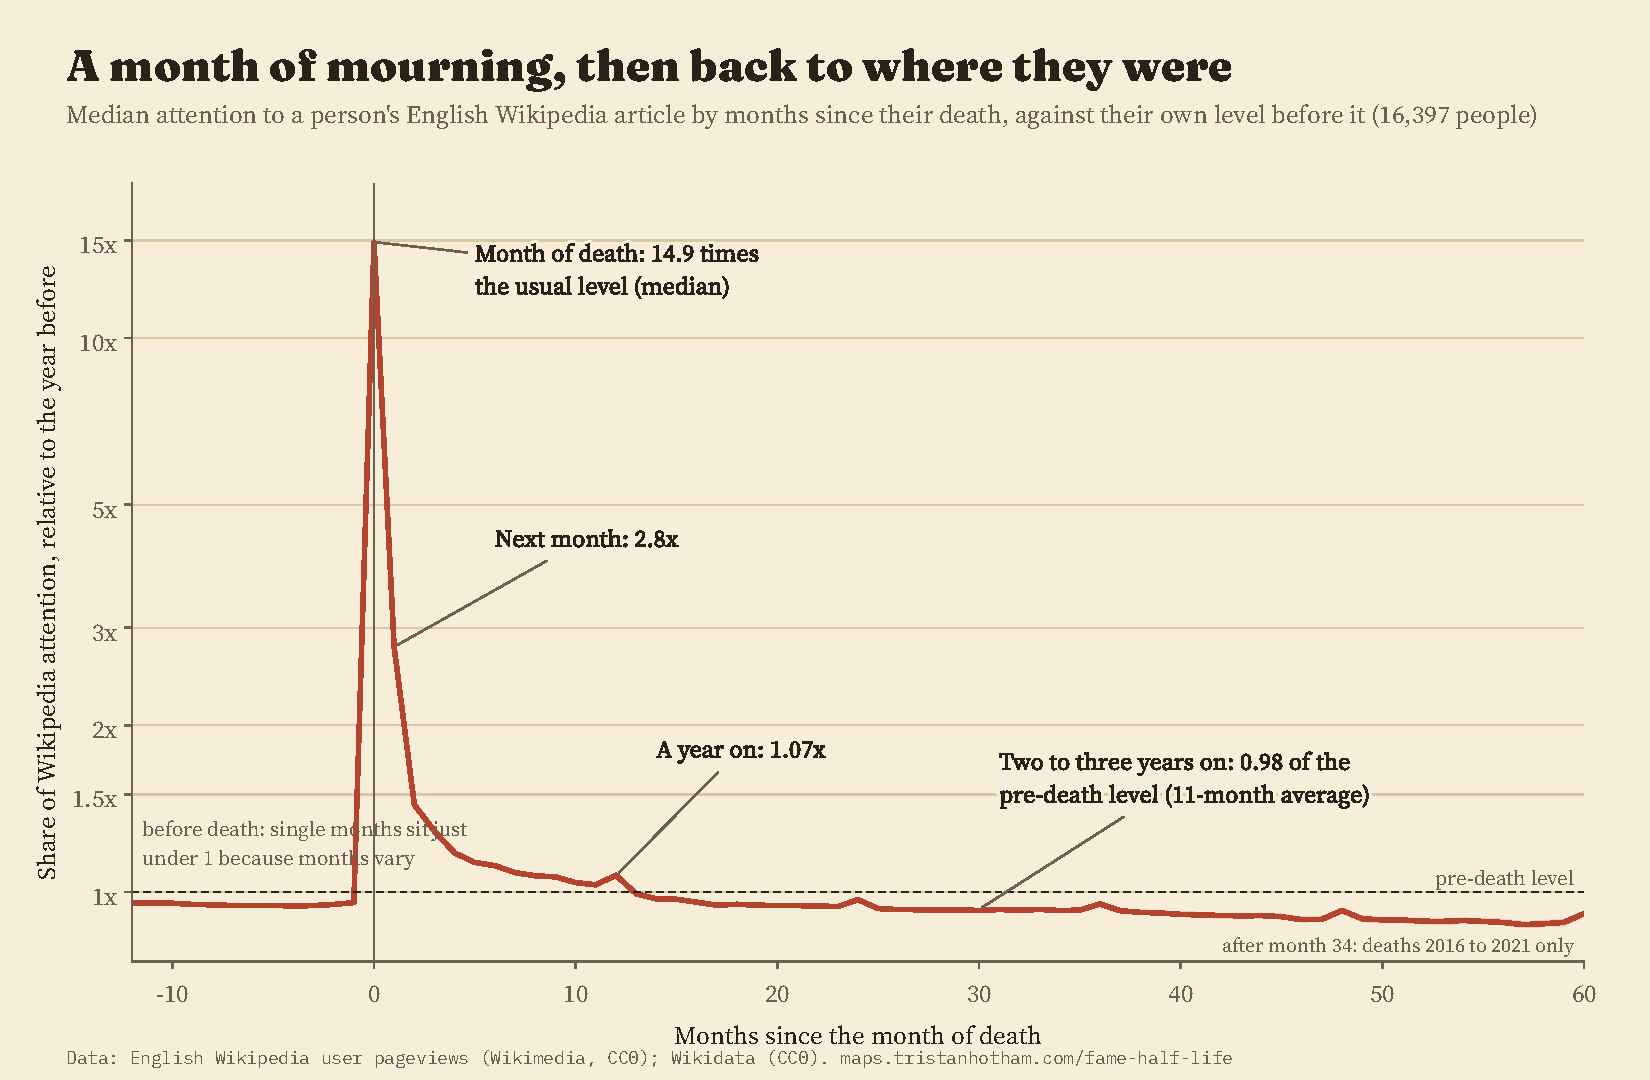
\includegraphics[width=\textwidth]{f_decay.pdf}
\caption{Median attention by months since death relative to each person's own baseline ($k = -12$ to $-2$), with 95\% bootstrap intervals; $N = 16,397$. Attention is the share of all English Wikipedia user views. Months 35 to 60 use deaths in 2016 to 2021 only.}\label{fig:decay}\end{figure}

\subsection{The shape of decay}
Table~\ref{tab:fits} and Figure~\ref{fig:fits} compare the three decay models. The two-phase model has the lowest AIC ($-$475, against $-$416 for the power law and $-$335 for the exponential), and it also wins when fitted only to $k = 1$ to 34, where every death is observed, and when fitted to the geometric-mean curve. In 100\% of 200 bootstrap resamples it has the lowest AIC. The fast component has a half-life of 11 days (95\% CI 11 to 12); the slow component has a half-life of 6.9 months (95\% CI 6.2 to 7.6); and the model settles at 0.90 (95\% CI 0.89 to 0.91) on the single-month scale, against a pre-death single-month level of about 0.95. At $k = 1$ the slow component already carries 20\% of the remaining excess.

Out of sample, however, the power law predicts the curve of deaths in 2020 to 2023 slightly better (log RMSE 0.0582) than the two-phase model (0.0595), with the exponential clearly worst (0.0675). By the pre-set criterion, H2 is therefore only partly supported: the two-phase model describes the curve best but does not generalise across cohorts better than a power law. The two are close, and both reject the single exponential, which decays too fast early and flattens too soon.

\begin{table}[tbp]\centering\small\caption{Decay models fitted to the median curve ($k = 1$ to 60 unless stated). AIC and BIC on log residuals; out-of-sample: fitted to deaths in 2016 to 2019, predicting 2020 to 2023 ($k = 1$ to 34), log RMSE.}\label{tab:fits}\begin{tabular}{lrrrrrrr}\toprule Model & Par. & AIC & BIC & AIC ($k\le34$) & AIC (geo. mean) & RMSE & Out-of-sample\\\midrule
exponential & 3 & $-$335.0 & $-$328.7 & $-$185.3 & $-$326.9 & 0.0583 & 0.0675\\
power law & 3 & $-$415.8 & $-$409.5 & $-$228.6 & $-$409.4 & 0.0298 & 0.0582\\
two$-$phase & 5 & $-$474.9 & $-$464.4 & $-$274.8 & $-$468.1 & 0.0176 & 0.0595\\
\bottomrule\end{tabular}\end{table}

\begin{figure}[tbp]\centering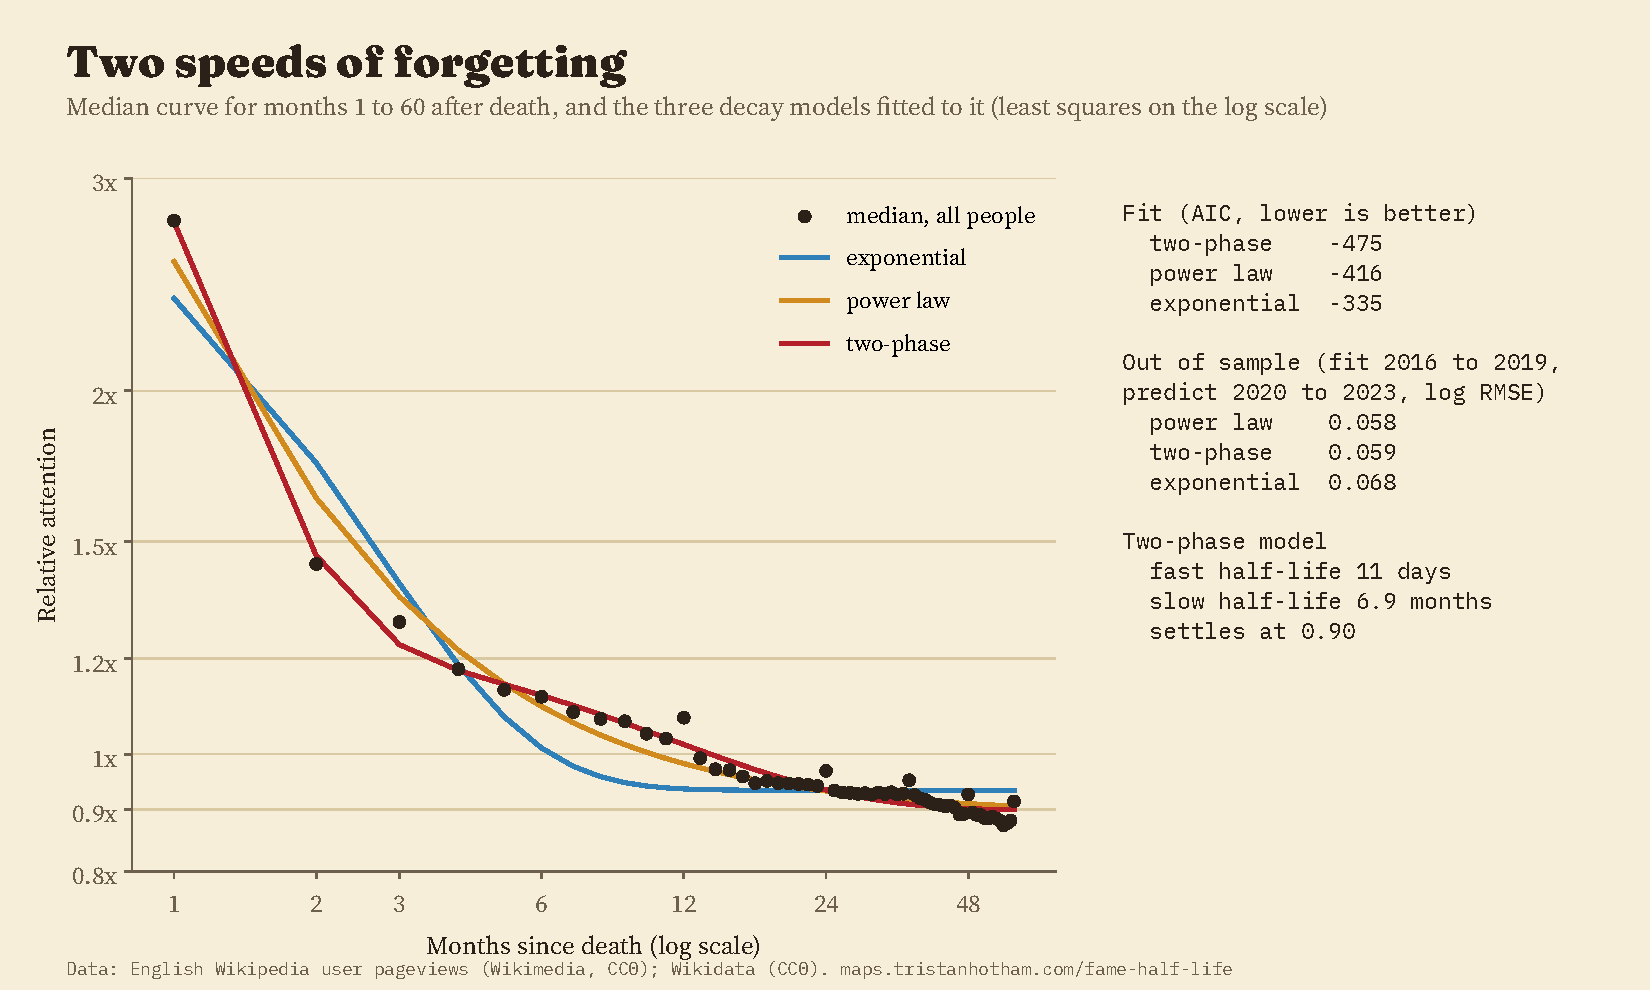
\includegraphics[width=\textwidth]{f_fits.pdf}
\caption{The median curve for $k = 1$ to 60 on log-log axes with the three fitted decay models.}\label{fig:fits}\end{figure}

The curve also shows small bumps at the anniversaries of the death (exploratory): at $k = 12$ the median is 6.0\% above the average of the months either side, at $k = 24$ 3.3\% and at $k = 36$ 2.7\%. These are consistent with commemorative attention on anniversaries, a form of the remembering triggers described by \citet{kanhabua2014}.

\subsection{The settling point}
Two to three years after death, the median LR is 0.978 (95\% CI 0.971 to 0.988), and 47.8\% of people are above their baseline. By the planned criterion, attention settles slightly below the pre-death level (H3). The spread is wide: the 10th and 90th percentiles of LR are 0.55 and 1.88. In raw views rather than shares, the median LR is 0.96, showing how much the decline of total traffic matters for the interpretation.

Is ``slightly below'' a loss or a gain? Attention to most articles drifts down over time even without a death. The placebo design measures that drift: over the year after a fake date 24 months before death, the median one-year ratio is 0.966 (95\% CI 0.960 to 0.972), against 1.062 after the real death. In an exploratory extension with a fake date 36 months before death, so that the fake long-run window coincides with the real baseline, the median no-death ratio is 0.952 (95\% CI 0.944 to 0.961) against 0.998 after the real death for the same 9,562 people. Relative to that drift, the typical person ends about 4.8\% above where they would otherwise have been (bootstrap 95\% interval 3.3 to 6.3; the median of the person-level ratio of real to placebo values is 6.5\% above). Both figures are exploratory and were not in the written plan. This comparison assumes that pre-death drift would have continued, which is not testable. Figure~\ref{fig:placebo} shows the real and placebo curves for the same people.

\begin{figure}[tbp]\centering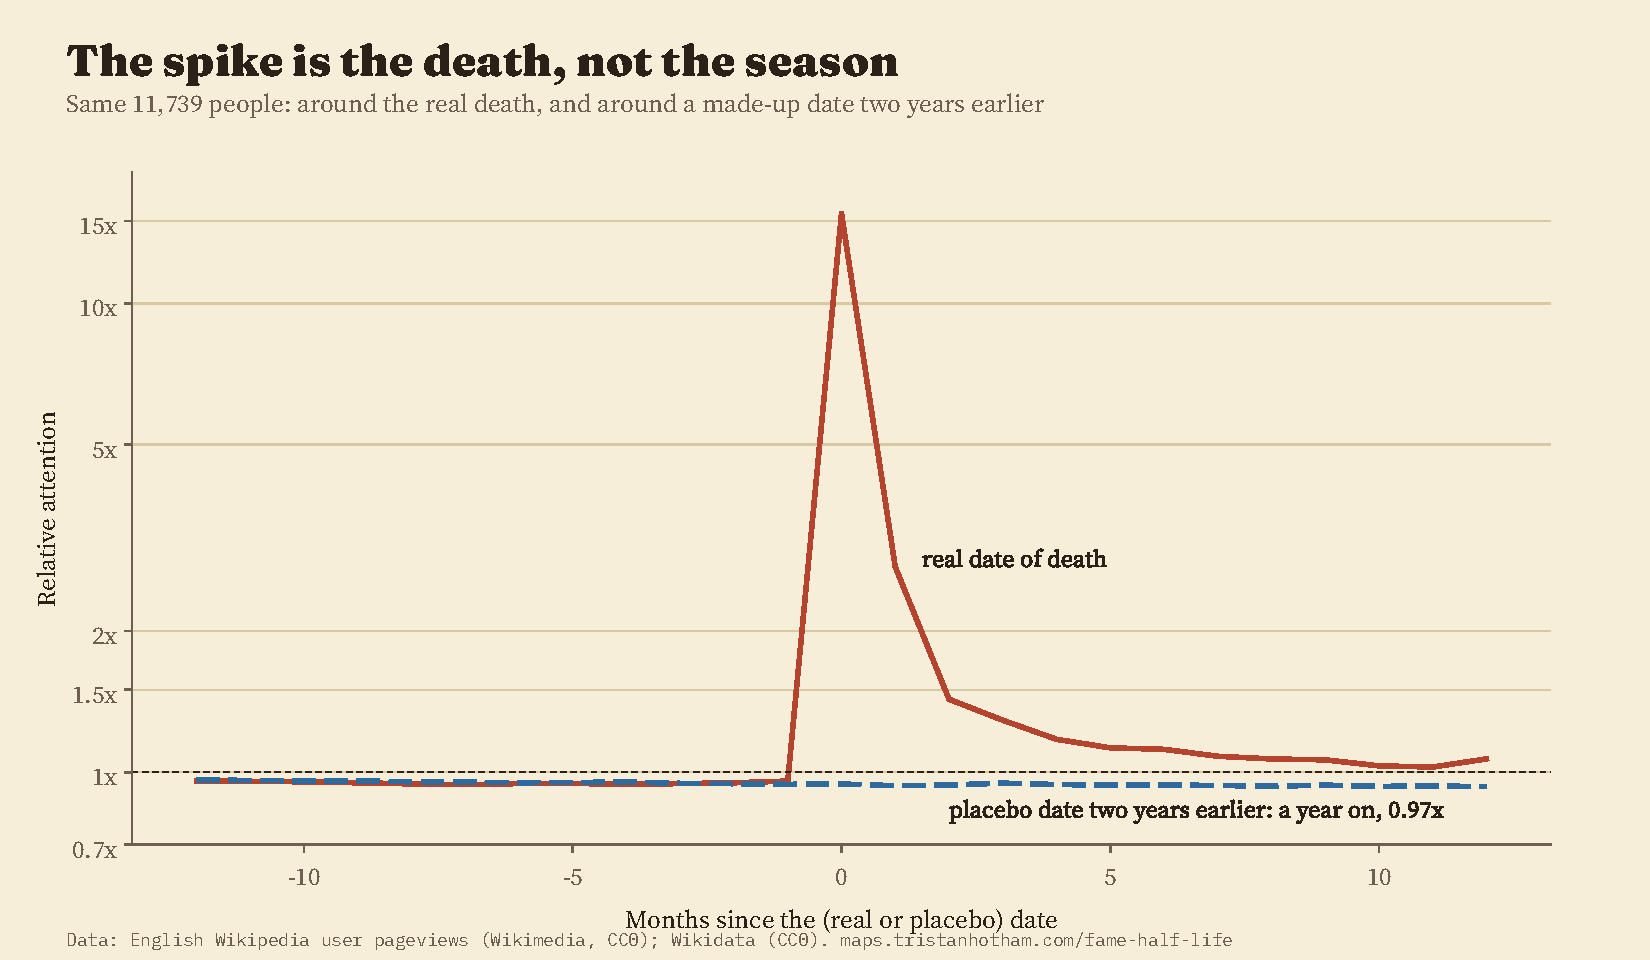
\includegraphics[width=\textwidth]{f_placebo.pdf}
\caption{Median attention around the real date of death and around a placebo date 24 months earlier, for the 11,739 people with enough history for both.}\label{fig:placebo}\end{figure}

\subsection{Who keeps attention}
Table~\ref{tab:main} reports the main regressions and Figure~\ref{fig:effects} summarises them. Occupational families differ jointly (Wald test $p < 10^{-10}$ for LR and for the peak). Every family keeps less long-run attention than performers, by 16\% for writers and artists, 31\% for sport, 24\% for politics and law, 24\% for science and academia and 34\% for religion. Descriptively (Table~\ref{tab:desc} and Figure~\ref{fig:families}), performers are the only family whose median LR is above one (1.10) and religious figures have the lowest (0.83). Peaks are ordered differently: journalists (48\%) and religious figures (30\%) have larger peaks than performers, scientists smaller ($-$32\%). In the language of \citet{candia2019}, deaths in some fields produce a large communicative response that is not converted into lasting attention.

\begin{figure}[tbp]\centering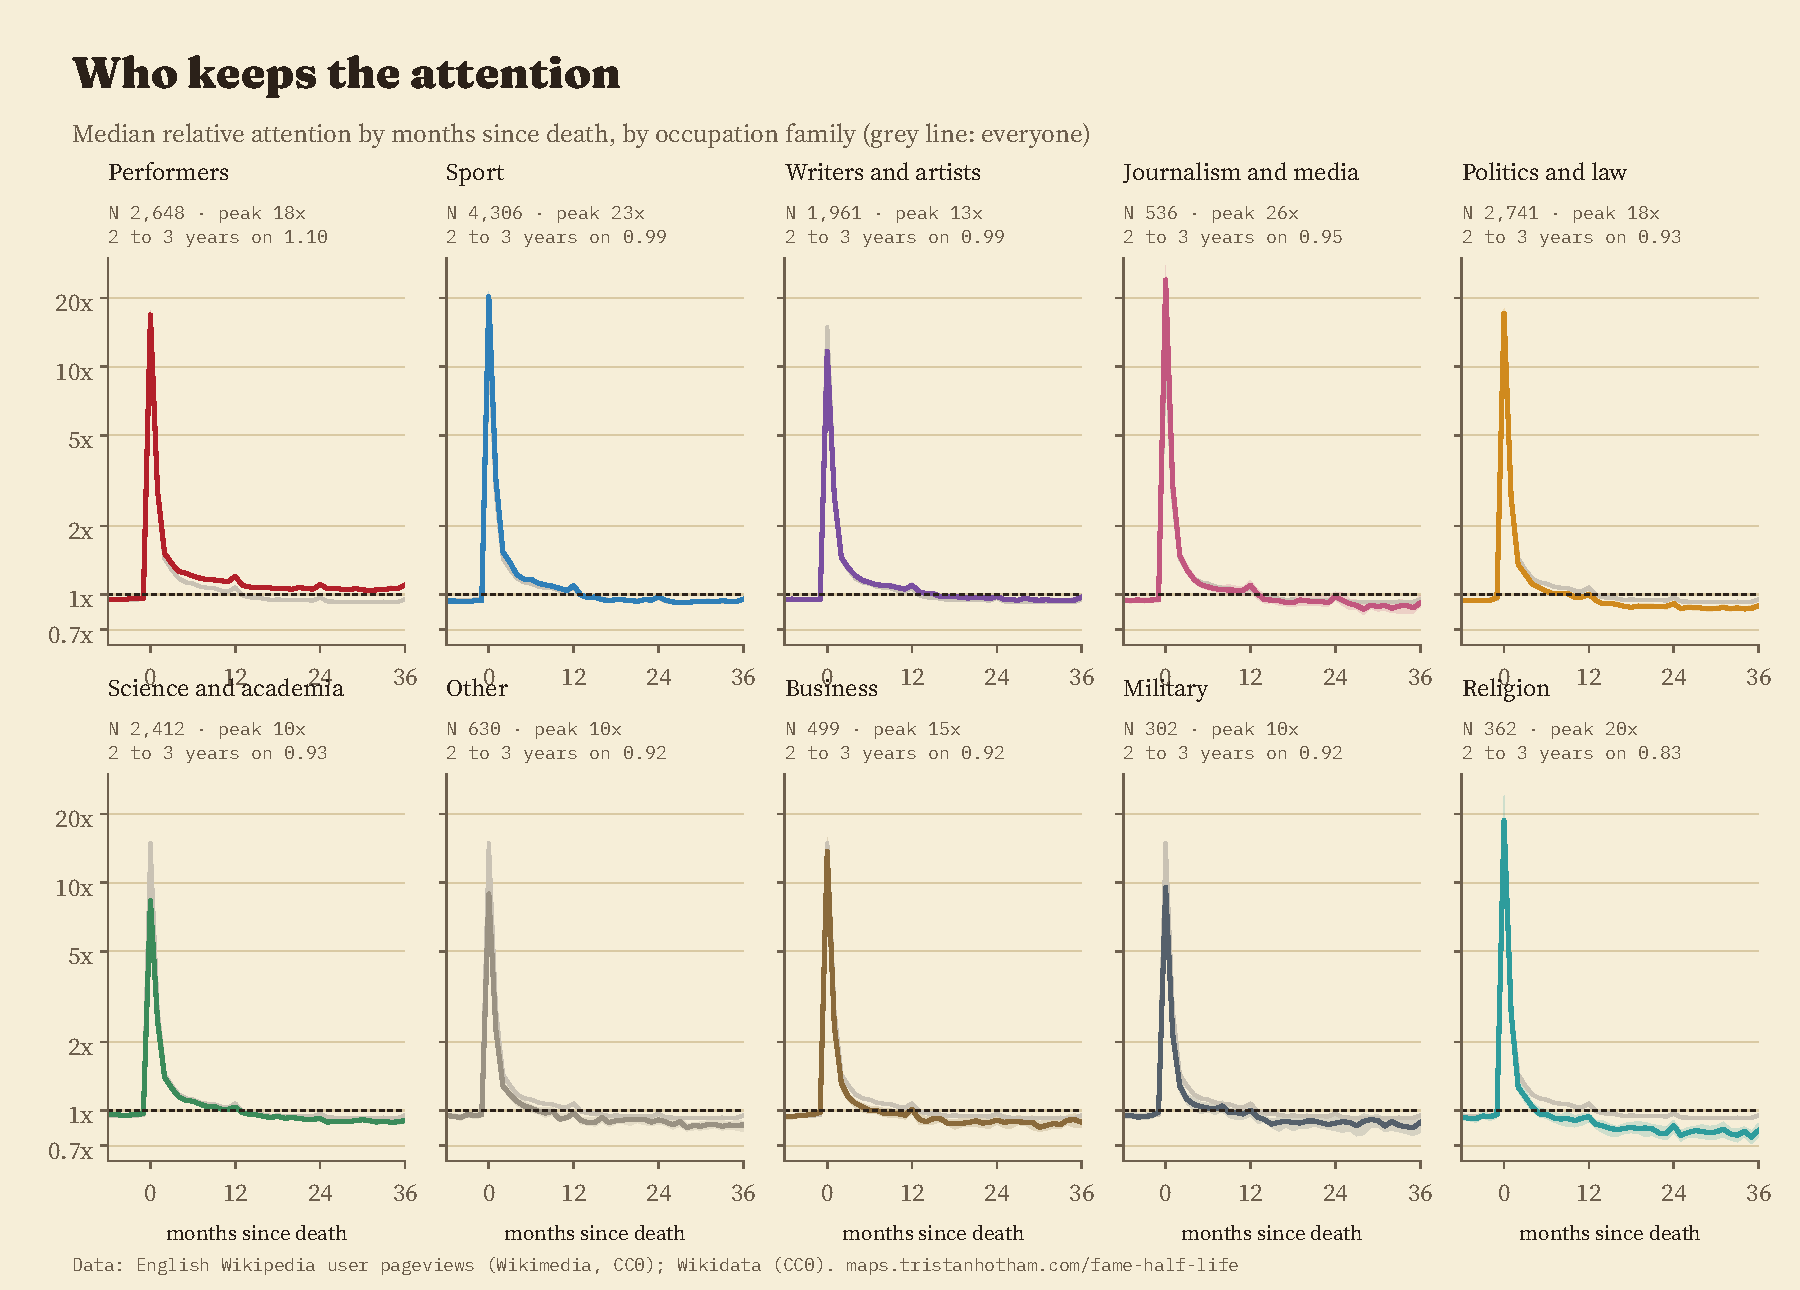
\includegraphics[width=\textwidth]{f_families.pdf}
\caption{Median attention by months since death for each occupation family (coloured) against everyone (grey).}\label{fig:families}\end{figure}

Age at death is the strongest correlate. Compared with people who died at 65 to 79, those who died under 50 have 347\% larger peaks (95\% CI 293 to 408) and 63\% more long-run attention (95\% CI 51 to 77); those who died at 90 or over have 15\% less (95\% CI 12 to 17). The gradient is monotone across the five bands (Figure~\ref{fig:age}). Descriptively, the median person who died under 50 peaked at 99 times their baseline and settled at 1.47; the median person who died at 90 or over peaked at 12 times and settled at 0.89. This matches the finding of \citet{west2021} that people who die young receive larger boosts in news and social media.

\begin{figure}[tbp]\centering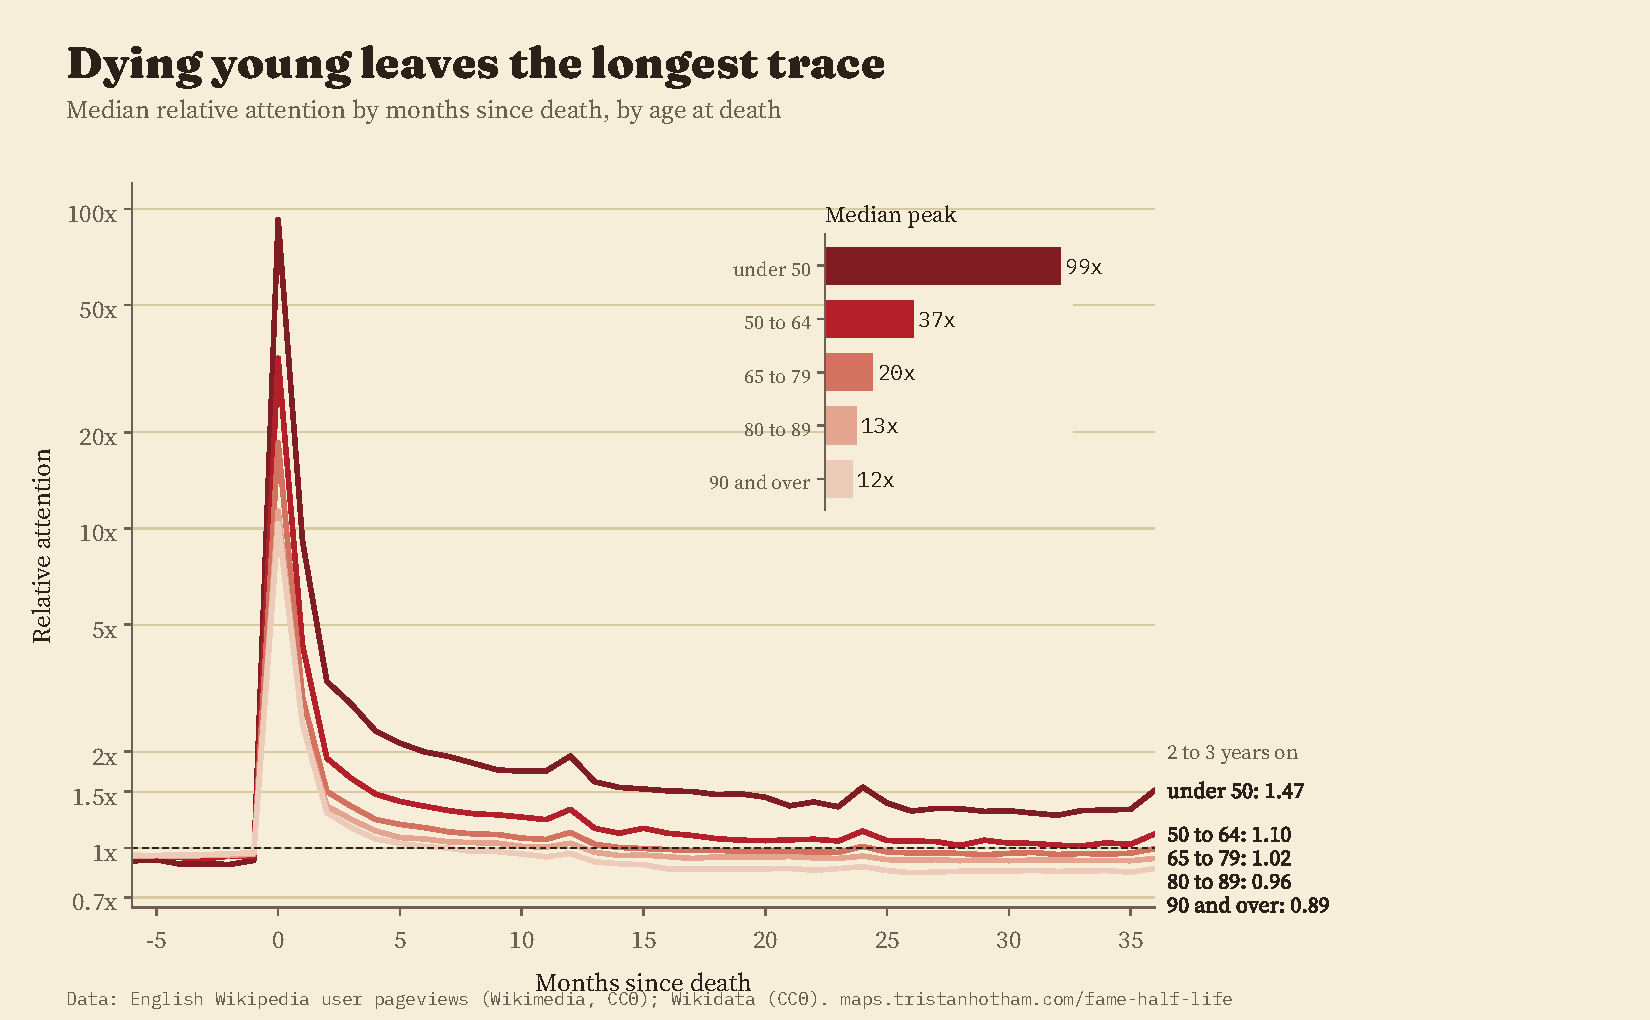
\includegraphics[width=\textwidth]{f_age.pdf}
\caption{Median attention by months since death by age at death; inset: median peak.}\label{fig:age}\end{figure}

Sitelinks, a proxy for international fame, go with larger peaks and more lasting attention: doubling sitelinks goes with 30\% larger peaks and 17\% more long-run attention (95\% CI 15 to 19), conditional on attention before death. Attention before death itself goes with smaller ratios (doubling it goes with 10\% lower LR), as the regression-to-the-mean argument above predicts.

Differences by sex are small. Women have a slightly higher raw median LR (1.02 against 0.97), but conditional on the other covariates their LR is 3\% lower (95\% CI 0 to 6). This estimate excludes zero in only 6 of 21 robustness checks and is 1.0\% without the baseline control, so I do not treat it as a finding. Citizens of English-speaking countries have smaller raw peaks on English Wikipedia (13.9 against 21.4), as one would expect when more readers already know them, and conditionally keep 23\% more long-run attention (95\% CI 19 to 27); but this conditional difference is 0.8\% without the baseline control and 6.3\% in the median regression, so it depends on how prior attention is handled and is not robust.

\begin{figure}[tbp]\centering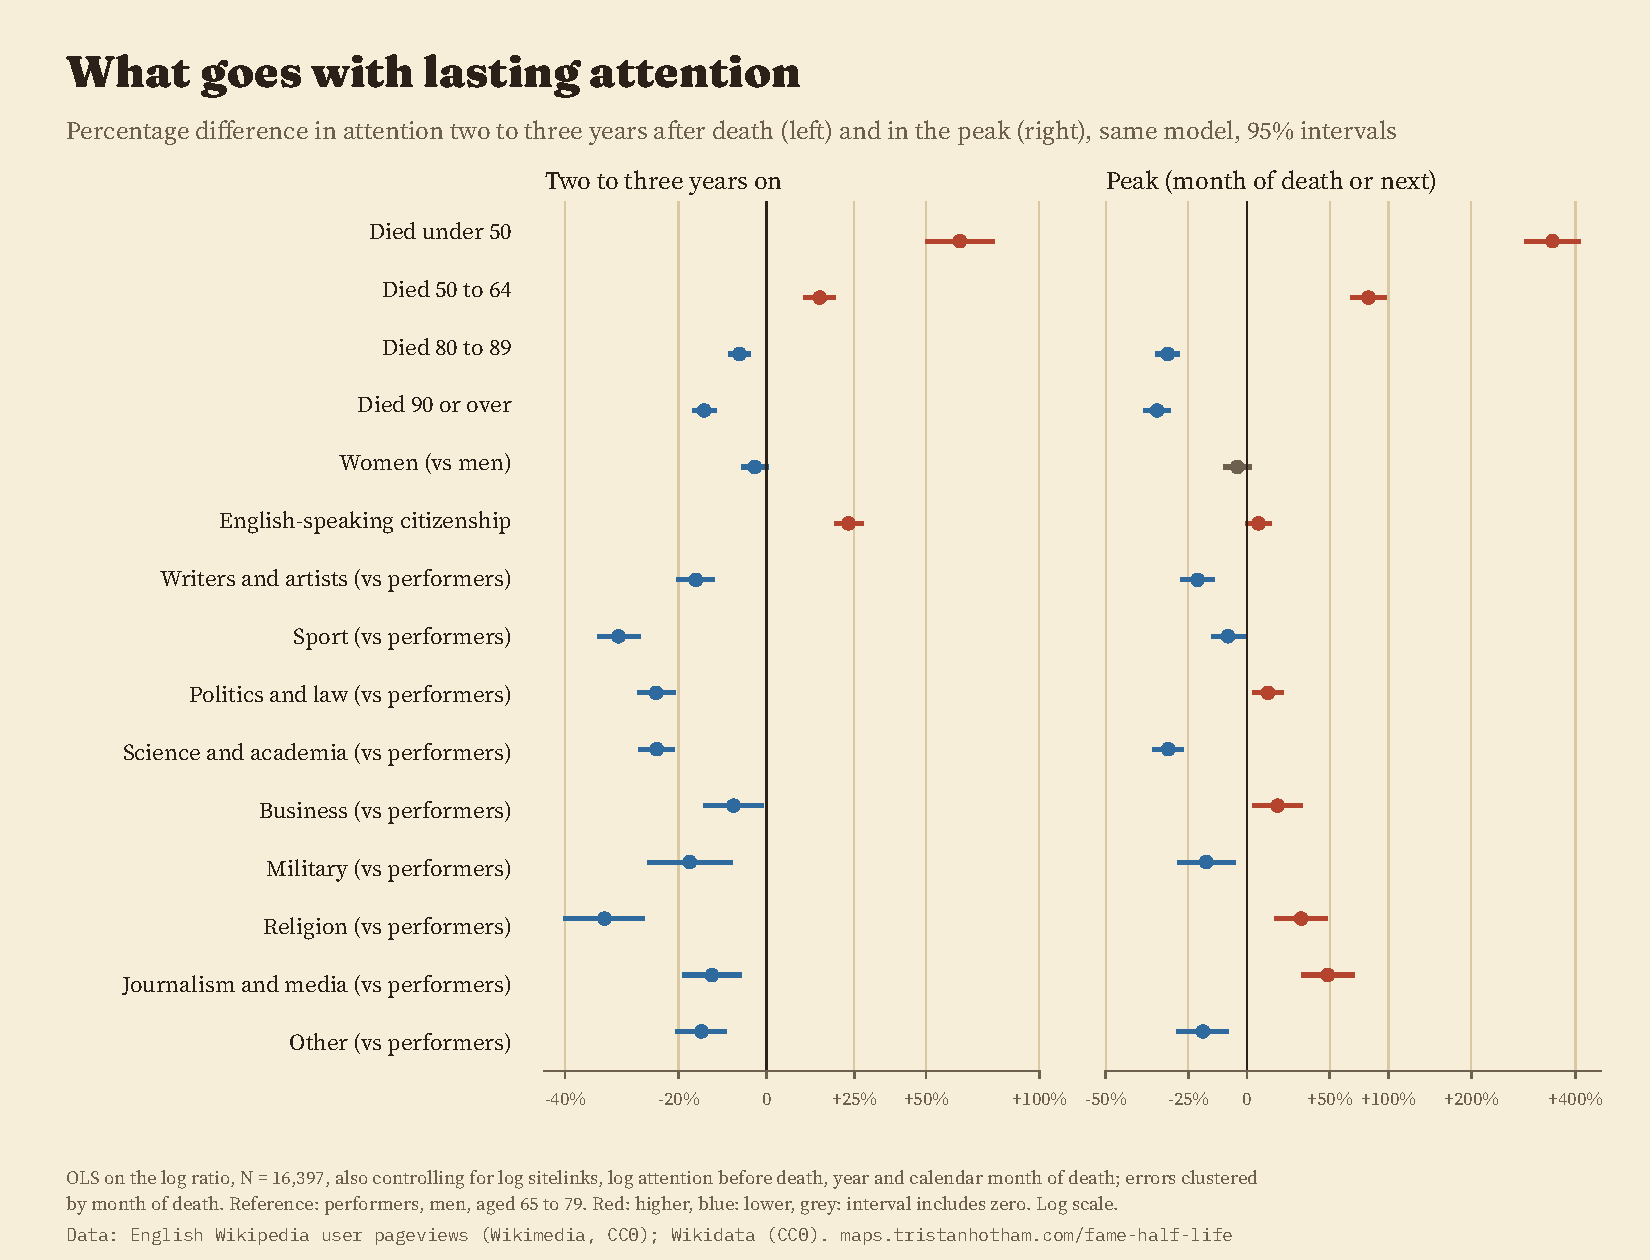
\includegraphics[width=\textwidth]{f_effects.pdf}
\caption{Percentage differences in long-run attention (left) and in the peak (right) from the main regressions, with 95\% intervals; $N = 16,397$.}\label{fig:effects}\end{figure}

\subsection{Placebo tests}
Table~\ref{tab:placebo} applies the main model to the placebo outcomes. The age differences do not appear at the placebo date: people under 50 have a placebo one-year ratio $-$3.1\% different from those aged 65 to 79 (95\% CI $-$8.4 to 2.5). Some occupational differences do: sportspeople's articles were already declining 13\% faster than performers' over a year without a death, and scientists' 11\% faster. English-speaking citizens' articles were drifting up relative to others' (6.8\%). The exploratory person-level difference between the real and placebo one-year ratios, which nets out each person's own drift, keeps the age gradient (under 50: 94\%; 90 and over: $-$19\%) and smaller but still negative gaps for sport ($-$8.6\%), politics ($-$12.2\%), religion ($-$21.9\%) and the military ($-$20.7\%). So part, but not all, of the occupational differences in long-run attention reflects trends that predate the deaths.

\begin{table}[tbp]\centering\scriptsize\caption{Placebo regressions (same model, same people): placebo peak and one-year ratio at a fake date 24 months before death; the real one-year ratio for the same people; and (exploratory) the person-level difference between real and placebo log one-year ratios. Percentage differences with 95\% intervals.}\label{tab:placebo}\setlength{\tabcolsep}{1.8pt}\resizebox{\textwidth}{!}{\begin{tabular}{p{4.0cm}rlllllll}\toprule Outcome & $N$ & Women & Under 50 & 90+ & English-sp. & Sport & Politics & Science\\\midrule
Placebo peak & 11,739 & $-$1 [$-$4, 1] & 0 [$-$6, 7] & 3 [1, 6] & 4 [1, 6] & $-$4 [$-$8, $-$1] & $-$1 [$-$5, 3] & $-$6 [$-$9, $-$3]\\
Placebo one-year ratio & 11,739 & $-$3 [$-$6, $-$0] & $-$3 [$-$8, 2] & 4 [1, 8] & 7 [4, 10] & $-$13 [$-$16, $-$9] & $-$8 [$-$11, $-$4] & $-$11 [$-$14, $-$8]\\
Real one-year ratio & 11,739 & 1 [$-$2, 4] & 88 [70, 107] & $-$16 [$-$18, $-$13] & 14 [11, 17] & $-$20 [$-$24, $-$17] & $-$19 [$-$22, $-$16] & $-$16 [$-$19, $-$12]\\
Real minus placebo (exploratory) & 11,739 & 4 [$-$0, 8] & 94 [70, 120] & $-$19 [$-$23, $-$15] & 6 [2, 11] & $-$9 [$-$14, $-$3] & $-$12 [$-$17, $-$7] & $-$6 [$-$10, $-$1]\\
\bottomrule\end{tabular}}\end{table}

\subsection{Articles created on death}\label{sec:posthumous}
Of the 26,236 people with a usable date of death and enough calendar history, 4,126 (15.7\%) had articles first read in the month of death or the month after. Most of these people appear to have become visible to English Wikipedia readers through their deaths, although some of these titles may have been moved at the time of death. Compared with the main sample, they are more often women (18.9\% against 15.0\%), more often in politics and law (23.9\% against 16.7\%) and religion, much less often sportspeople (9.8\% against 26.3\%), and have fewer sitelinks (median 3 against 5). Their first full month had a median of 137 views; two to three years later the median was 30.5 a month, about 23\% of the first full month.

\subsection{Countries}
Figure~\ref{fig:map} maps the median LR by country of citizenship for the 61 citizenships with at least 30 people in the main sample. The United States (5,044 people) has a median of 0.97 and the United Kingdom (1,573) 0.95. Several countries outside the English-speaking world have medians above one, in line with the negative coefficient on attention before death (people with less English Wikipedia attention before death gain more relative to it). Country differences are descriptive; many rest on small numbers and the confidence intervals, reported in the released data, are wide.

\begin{figure}[tbp]\centering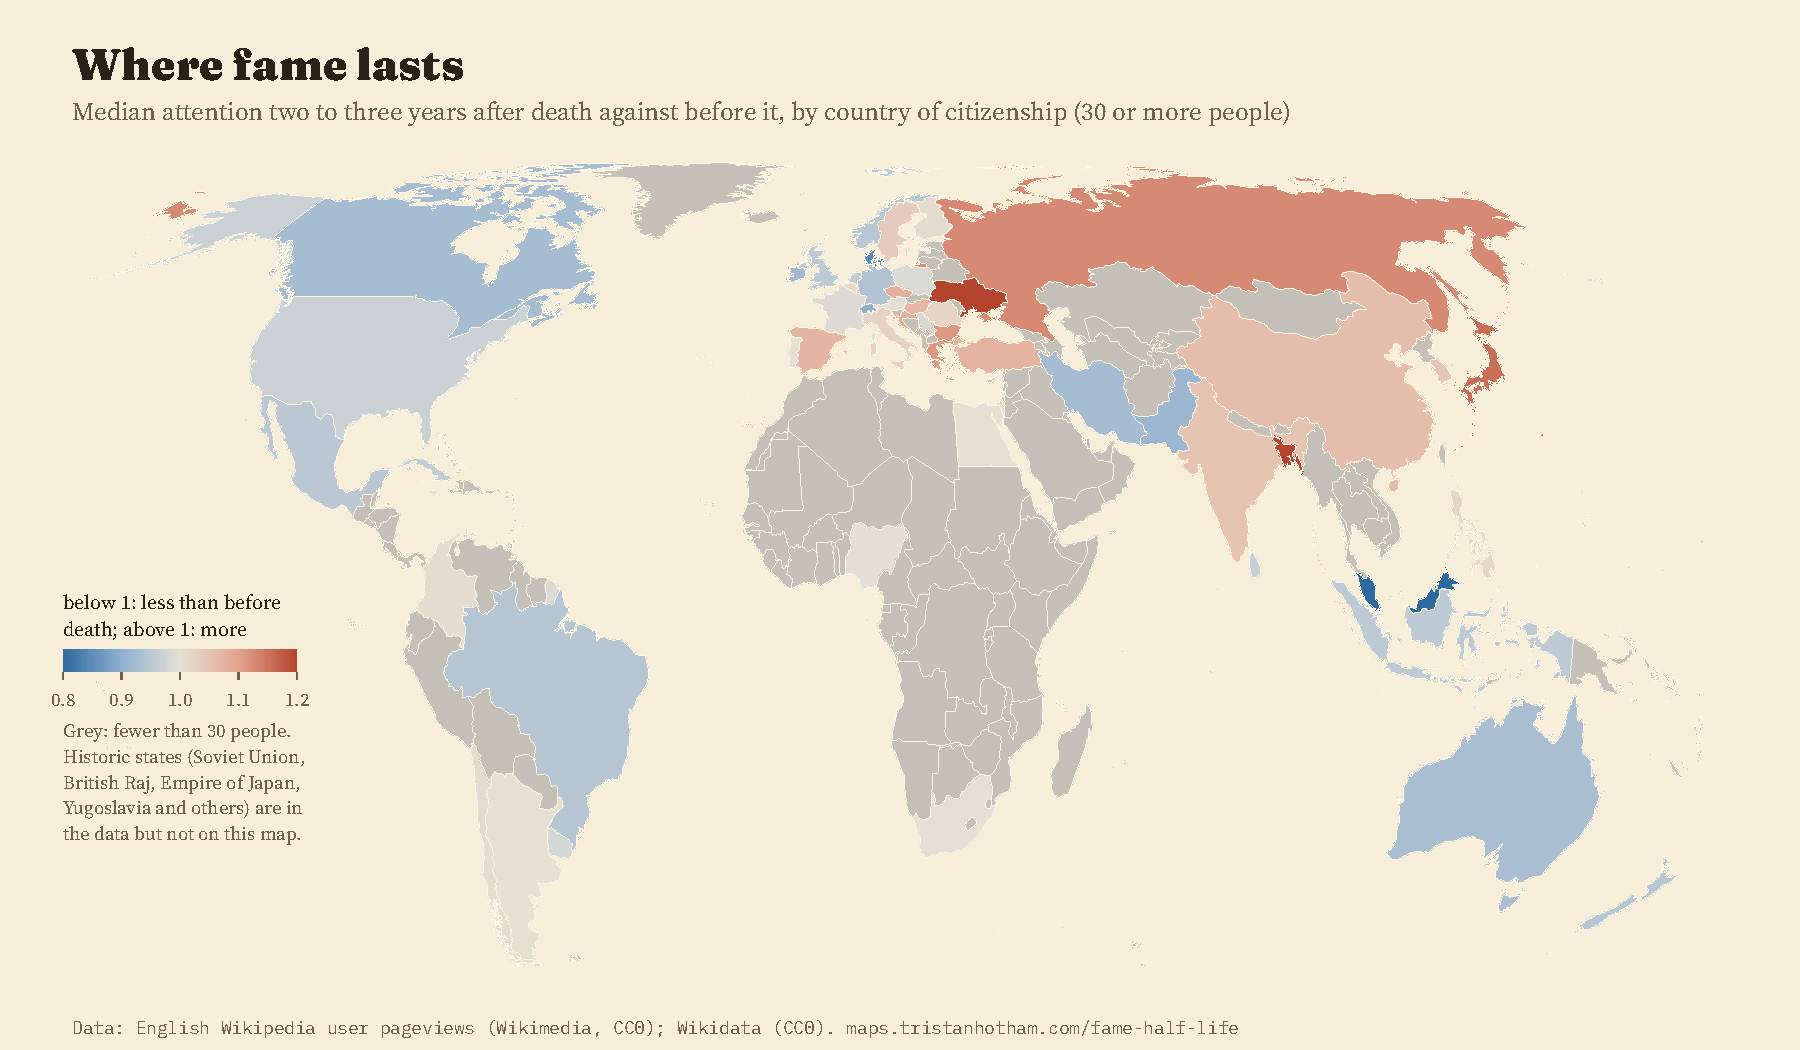
\includegraphics[width=\textwidth]{f_map.pdf}
\caption{Median long-run ratio by country of citizenship (30 or more people). Historic states recorded as citizenship in Wikidata, such as the Soviet Union, are not shown.}\label{fig:map}\end{figure}

\section{Robustness}\label{sec:robust}
Table~\ref{tab:robust} reports the 21 pre-specified robustness checks for the long-run model. The age gradient is stable: the under-50 difference ranges from 45\% to 68\% and the 90-and-over difference from $-$15\% to $-$12\%, with intervals excluding zero in every check. The occupational differences keep their signs and significance in every check, although they are smaller in the median regression (sport $-$17\%). The English-speaking difference ranges from 6\% to 24\%. The difference for women excludes zero in only 6 checks. Leaving out each occupation family in turn leaves the age and sex estimates essentially unchanged (Appendix Table~\ref{tab:lofo}). The conclusions about the aggregate curve do not depend on the bot rule: only 71 main-sample series have a bot-like spike in the baseline. Two of the pre-specified checks cannot change the coefficients: heteroskedasticity-robust errors change only the intervals, and the raw-views check gives coefficients identical to the main model by construction, because log LR in raw views differs from log LR in shares by a term that depends only on the month of death, which the year and calendar-month fixed effects together absorb. Normalisation by total traffic therefore matters for the level of the curve (median LR 0.98 in shares, 0.96 in raw views), not for the comparisons between groups.

\subsection{Further checks (exploratory, added at review)}
Four further checks were added after an independent review and are exploratory. First, regression to the mean: replacing the log baseline control, which shares its measurement noise with the denominator of LR, by log attention measured in an earlier, separate window ($k = -24$ to $-13$; $N = 14,510$) leaves the age gradient almost unchanged (under 50: 59\%, 95\% CI 46 to 74; 90 and over: $-$15\%), shrinks the English-speaking difference to 14\% (95\% CI 11 to 18; 19\% with the main control in the same people) and gives $-$1.7\% for women (95\% CI $-$4.3 to 1.0). Second, clustering by country of citizenship (236 clusters) instead of month of death widens the English-speaking interval (16 to 31) and the interval for women ($-$6.2 to 0.6) but leaves the age intervals clear of zero. Third, 182 main-sample series look like titles that were redirects before the article moved onto them (under five views a month in the baseline, or no rise at death with LR above 5); such a series measures the title, not the person. Dropping them leaves the median LR at 0.97 and the age gradient intact (under 50: 60\%), lowers the English-speaking difference to 16\% and the difference for women to $-$1.1\% (95\% CI $-$3.4 to 1.3). Fourth, the composition of the articles dropped because they were first read two or more months after death is reported in Section~\ref{sec:data}. Together these checks support the age gradient and the occupational ordering and confirm that the estimates for women and for English-speaking citizenship should not be treated as findings.

\begin{table}[tbp]\centering\scriptsize\caption{Robustness checks for log LR. Percentage differences with 95\% intervals for women (vs men), death under 50 and at 90 or over (vs 65 to 79), English-speaking citizenship, and sport, politics and law, and science and academia (vs performers).}\label{tab:robust}\setlength{\tabcolsep}{1.8pt}\resizebox{\textwidth}{!}{\begin{tabular}{p{4.4cm}rlllllll}\toprule Check & $N$ & Women & Under 50 & 90+ & English-sp. & Sport & Politics & Science\\\midrule
\multicolumn{9}{l}{\textit{Alternative specification}}\\
\quad Median regression (q = 0.5) & 16,397 & $-$0 [$-$2, 2] & 45 [40, 51] & $-$12 [$-$14, $-$11] & 6 [4, 8] & $-$17 [$-$19, $-$15] & $-$17 [$-$19, $-$15] & $-$15 [$-$17, $-$13]\\
\quad OLS, log LR winsorised 1/99 & 16,397 & $-$1 [$-$3, 1] & 58 [48, 70] & $-$13 [$-$15, $-$12] & 16 [13, 19] & $-$25 [$-$28, $-$22] & $-$21 [$-$24, $-$18] & $-$20 [$-$23, $-$18]\\
\quad Robust (HC1) standard errors & 16,397 & $-$3 [$-$6, 0] & 63 [51, 76] & $-$15 [$-$17, $-$12] & 23 [19, 27] & $-$31 [$-$34, $-$28] & $-$24 [$-$28, $-$21] & $-$24 [$-$27, $-$21]\\
\multicolumn{9}{l}{\textit{Outliers}}\\
\quad Drop top 1\% by peak & 16,233 & $-$2 [$-$5, 0] & 47 [38, 58] & $-$14 [$-$16, $-$12] & 18 [14, 21] & $-$27 [$-$30, $-$23] & $-$22 [$-$25, $-$19] & $-$22 [$-$24, $-$19]\\
\quad Drop top 1\% by baseline attention & 16,233 & $-$3 [$-$5, 0] & 62 [49, 76] & $-$14 [$-$16, $-$12] & 23 [19, 27] & $-$31 [$-$35, $-$27] & $-$24 [$-$28, $-$21] & $-$24 [$-$27, $-$21]\\
\multicolumn{9}{l}{\textit{Leave one out}}\\
\quad Leave out US citizens & 11,353 & $-$5 [$-$8, $-$2] & 58 [44, 73] & $-$14 [$-$17, $-$11] & 19 [15, 24] & $-$34 [$-$38, $-$30] & $-$23 [$-$27, $-$19] & $-$23 [$-$27, $-$19]\\
\quad Leave out deaths in 2016 & 14,915 & $-$4 [$-$6, $-$1] & 62 [48, 77] & $-$15 [$-$17, $-$13] & 24 [20, 28] & $-$32 [$-$36, $-$28] & $-$25 [$-$28, $-$21] & $-$25 [$-$28, $-$22]\\
\quad Leave out deaths in 2017 & 14,632 & $-$3 [$-$6, $-$0] & 64 [50, 78] & $-$14 [$-$17, $-$12] & 23 [19, 27] & $-$31 [$-$34, $-$27] & $-$25 [$-$28, $-$21] & $-$24 [$-$27, $-$21]\\
\quad Leave out deaths in 2018 & 14,548 & $-$2 [$-$5, 0] & 64 [51, 78] & $-$15 [$-$17, $-$12] & 24 [20, 28] & $-$30 [$-$33, $-$26] & $-$23 [$-$26, $-$20] & $-$24 [$-$27, $-$20]\\
\quad Leave out deaths in 2019 & 14,400 & $-$3 [$-$6, 0] & 61 [47, 75] & $-$14 [$-$16, $-$12] & 24 [20, 28] & $-$30 [$-$34, $-$27] & $-$23 [$-$27, $-$20] & $-$24 [$-$27, $-$20]\\
\quad Leave out deaths in 2020 & 13,920 & $-$2 [$-$5, 0] & 62 [49, 77] & $-$14 [$-$16, $-$11] & 23 [19, 27] & $-$32 [$-$35, $-$28] & $-$25 [$-$28, $-$21] & $-$24 [$-$27, $-$20]\\
\quad Leave out deaths in 2021 & 13,876 & $-$3 [$-$6, 0] & 67 [53, 83] & $-$14 [$-$17, $-$12] & 23 [19, 28] & $-$32 [$-$35, $-$28] & $-$25 [$-$29, $-$22] & $-$25 [$-$28, $-$21]\\
\quad Leave out deaths in 2022 & 14,335 & $-$3 [$-$6, $-$0] & 64 [50, 79] & $-$15 [$-$17, $-$13] & 22 [18, 27] & $-$32 [$-$36, $-$28] & $-$25 [$-$28, $-$21] & $-$25 [$-$28, $-$22]\\
\quad Leave out deaths in 2023 & 14,153 & $-$3 [$-$6, 0] & 64 [50, 80] & $-$15 [$-$17, $-$12] & 22 [18, 27] & $-$32 [$-$35, $-$27] & $-$23 [$-$27, $-$20] & $-$24 [$-$28, $-$21]\\
\multicolumn{9}{l}{\textit{Measurement}}\\
\quad Raw views, not share of enwiki & 16,397 & $-$3 [$-$6, $-$0] & 63 [51, 77] & $-$15 [$-$17, $-$12] & 23 [19, 27] & $-$31 [$-$35, $-$28] & $-$24 [$-$28, $-$21] & $-$24 [$-$27, $-$21]\\
\quad Baseline months -6 to -2 & 16,374 & $-$1 [$-$4, 1] & 68 [54, 83] & $-$14 [$-$16, $-$12] & 18 [15, 22] & $-$27 [$-$30, $-$24] & $-$22 [$-$25, $-$19] & $-$22 [$-$24, $-$19]\\
\quad Long-run window months 18 to 30 & 16,397 & $-$2 [$-$5, 0] & 67 [54, 80] & $-$15 [$-$17, $-$13] & 23 [19, 27] & $-$31 [$-$34, $-$27] & $-$24 [$-$27, $-$20] & $-$23 [$-$26, $-$20]\\
\quad Full 11-month baseline only & 15,749 & $-$3 [$-$6, $-$0] & 63 [49, 77] & $-$15 [$-$17, $-$12] & 23 [19, 27] & $-$32 [$-$35, $-$28] & $-$25 [$-$28, $-$21] & $-$25 [$-$28, $-$22]\\
\quad Drop series with bot-like baseline spikes & 16,326 & $-$3 [$-$5, 0] & 65 [52, 79] & $-$14 [$-$17, $-$12] & 22 [19, 26] & $-$31 [$-$34, $-$27] & $-$24 [$-$27, $-$20] & $-$24 [$-$27, $-$21]\\
\quad Occupation: first in file order & 16,397 & $-$3 [$-$6, $-$0] & 63 [51, 77] & $-$15 [$-$17, $-$12] & 23 [19, 27] & $-$31 [$-$35, $-$28] & $-$24 [$-$28, $-$21] & $-$24 [$-$27, $-$21]\\
\quad Include 1 January dates of death & 17,751 & $-$2 [$-$5, 0] & 61 [48, 75] & $-$15 [$-$17, $-$13] & 22 [18, 25] & $-$30 [$-$34, $-$27] & $-$24 [$-$27, $-$21] & $-$24 [$-$27, $-$21]\\
\midrule Main model & 16,397 & $-$3 [$-$6, $-$0] & 63 [51, 77] & $-$15 [$-$17, $-$12] & 23 [19, 27] & $-$31 [$-$35, $-$28] & $-$24 [$-$28, $-$21] & $-$24 [$-$27, $-$21]\\
\bottomrule\end{tabular}}\end{table}

\section{Discussion}\label{sec:disc}
\subsection{What the curve says}
For the typical notable person, death produces a month of intense attention, mostly gone within weeks, and a slower tail that has largely returned to the old level after two or three years. In aggregate the picture is different, because the largest and most lasting gains belong to the most famous: the total attention of the sample, two to three years on, is 1.12 times its baseline. Both statements are true, and which one matters depends on whether one asks about people or about the attention economy.

The two-phase shape fits the idea of communicative and cultural memory \citep{assmann1995,candia2019}, but the time scales here are far shorter than in \citet{candia2019}, whose communicative component for biographies lasts decades. A month-scale spike and a slow component with a half-life of months describe news and its aftermath, not the passing of generations. The power law's better out-of-sample performance is a reminder that functional forms fitted to aggregate curves are hard to distinguish \citep{rubin1996}; aggregates of individual decays with different rates can look like a power law even when no individual curve is one, so the aggregate shape need not describe any single person.

\subsection{Who is remembered}
The age gradient is the most robust result and it is not explained by pre-existing trends. Deaths of younger people are more often sudden and more often of people still active, both of which plausibly raise both the surprise and the sense of an unfinished career. The data cannot separate these. The occupational ordering, with performers at the top, is consistent with \citet{west2021}'s finding that artists receive larger long-term boosts, and with the possibility, which these data cannot test, that performers' recordings and films continue to circulate after death. That part of the occupational gap predates the deaths is a caution for any study that compares groups after an event without a pre-event trend.

The absence of a robust difference by sex should be read carefully. It describes the ratio of attention after death to attention before, among people who already had articles. It says nothing about the well-documented gaps in coverage \citep{wagner2015,wagner2016,konieczny2018}, which operate at the stage of inclusion; indeed, women are over-represented among those whose articles were created only on their deaths.

\subsection{Limitations}
Several limitations follow from the data. First, pageviews measure looking up, not remembering, valuing or grieving. Second, English Wikipedia is one audience, global but disproportionately anglophone, and patterns for other languages may differ \citep{lemmerich2019}. Third, Wikidata supplies one sampled occupation and one sampled citizenship per person, and cause of death is not available; the age effect may partly be an effect of sudden death. Fourth, articles renamed or written after the death drop out of the before-and-after sample, and this dropout is not random (it removes relatively more women and non-English-speaking citizens); a small number of retained titles appear to have been redirects before the death; and the 1 January rule removes year-precision dates. All three are documented, and the last two are tested. Fifth, the user agent excludes identified bots but not all automated traffic; series with bot-like spikes are few and excluding them changes nothing. Sixth, the follow-up after 34 months comes from earlier cohorts only. Finally, the regression mixes people across the period 2016 to 2023, which includes the COVID-19 pandemic and its excess mortality; year-of-death fixed effects absorb level differences but not differences in the composition of who died.

\section{Conclusion}
Fame decays fast after death. The typical notable person's English Wikipedia article is read about 16 times as much as usual at the time of death, loses the bulk of that surge within weeks, and two to three years later is read at about the same share as before, perhaps slightly more than the downward drift before death would have predicted. Lasting gains are largest for people who die young and for performers, and, in absolute terms, for the most famous. The data and code released with this paper allow the same curve to be measured for other languages, periods and events.

\section*{Data availability statement}
Data and code: Zenodo DOI https://doi.org/10.5281/zenodo.24095452. The interactive page is at \url{https://maps.tristanhotham.com/fame-half-life/} and the repository at \url{https://github.com/Tristan-Hotham/fame-half-life}. Person-level measures (no raw series) and aggregate curves are released under CC BY 4.0; the underlying pageviews (Wikimedia) and Wikidata are CC0.

\section*{AI statement}
I wrote the text, with drafting and editing assistance from Claude (Anthropic), which also helped prepare the analysis code. I reviewed and checked all text and results.

\begin{thebibliography}{99}
\bibitem[Abadie et al.(2023)]{abadie2023} Abadie, A., Athey, S., Imbens, G. W. and Wooldridge, J. M. (2023) When should you adjust standard errors for clustering? \textit{Quarterly Journal of Economics} 138(1), 1 to 35.
\bibitem[Assmann and Czaplicka(1995)]{assmann1995} Assmann, J. and Czaplicka, J. (1995) Collective memory and cultural identity. \textit{New German Critique} 65, 125 to 133.
\bibitem[Cameron and Miller(2015)]{cameron2015} Cameron, A. C. and Miller, D. L. (2015) A practitioner's guide to cluster-robust inference. \textit{Journal of Human Resources} 50(2), 317 to 372.
\bibitem[Candia et al.(2019)]{candia2019} Candia, C., Jara-Figueroa, C., Rodriguez-Sickert, C., Barabási, A.-L. and Hidalgo, C. A. (2019) The universal decay of collective memory and attention. \textit{Nature Human Behaviour} 3(1), 82 to 91. doi:10.1038/s41562-018-0474-5.
\bibitem[Crane and Sornette(2008)]{crane2008} Crane, R. and Sornette, D. (2008) Robust dynamic classes revealed by measuring the response function of a social system. \textit{Proceedings of the National Academy of Sciences} 105(41), 15649 to 15653. doi:10.1073/pnas.0803685105.
\bibitem[Ekelund et al.(2000)]{ekelund2000} Ekelund, R. B., Ressler, R. W. and Watson, J. K. (2000) The ``death-effect'' in art prices: a demand-side exploration. \textit{Journal of Cultural Economics} 24(4), 283 to 300. doi:10.1023/A:1007618221648.
\bibitem[García-Gavilanes et al.(2017)]{garciagavilanes2017} García-Gavilanes, R., Mollgaard, A., Tsvetkova, M. and Yasseri, T. (2017) The memory remains: understanding collective memory in the digital age. \textit{Science Advances} 3(4), e1602368. doi:10.1126/sciadv.1602368.
\bibitem[Gergaud et al.(2016)]{gergaud2016} Gergaud, O., Laouenan, M. and Wasmer, E. (2016) A brief history of human time: exploring a database of ``notable people''. Sciences Po Economics Discussion Paper, HAL hal-03393214.
\bibitem[Graells-Garrido et al.(2015)]{graellsgarrido2015} Graells-Garrido, E., Lalmas, M. and Menczer, F. (2015) First women, second sex: gender bias in Wikipedia. In \textit{Proceedings of the 26th ACM Conference on Hypertext and Social Media}, 165 to 174. doi:10.1145/2700171.2791036.
\bibitem[Halbwachs(1992)]{halbwachs1992} Halbwachs, M. (1992) \textit{On Collective Memory}, ed. and trans. L. A. Coser. Chicago: University of Chicago Press.
\bibitem[Kanhabua et al.(2014)]{kanhabua2014} Kanhabua, N., Nguyen, T. N. and Niederée, C. (2014) What triggers human remembering of events? A large-scale analysis of catalysts for collective memory in Wikipedia. In \textit{Proceedings of the 14th ACM/IEEE-CS Joint Conference on Digital Libraries}, 341 to 350.
\bibitem[Keegan and Brubaker(2015)]{keegan2015} Keegan, B. C. and Brubaker, J. R. (2015) `Is' to `was': coordination and commemoration in posthumous activity on Wikipedia biographies. In \textit{Proceedings of the 18th ACM Conference on Computer Supported Cooperative Work and Social Computing (CSCW)}, 533 to 546. doi:10.1145/2675133.2675238.
\bibitem[Koenker and Bassett(1978)]{koenker1978} Koenker, R. and Bassett, G. (1978) Regression quantiles. \textit{Econometrica} 46(1), 33 to 50.
\bibitem[Konieczny and Klein(2018)]{konieczny2018} Konieczny, P. and Klein, M. (2018) Gender gap through time and space: a journey through Wikipedia biographies via the Wikidata Human Gender Indicator. \textit{New Media and Society} 20(12), 4608 to 4633. doi:10.1177/1461444818779080.
\bibitem[Laouenan et al.(2022)]{laouenan2022} Laouenan, M., Bhargava, P., Eyméoud, J.-B., Gergaud, O., Plique, G. and Wasmer, E. (2022) A cross-verified database of notable people, 3500BC to 2018AD. \textit{Scientific Data} 9, 290. doi:10.1038/s41597-022-01369-4.
\bibitem[Lehmann et al.(2012)]{lehmann2012} Lehmann, J., Gonçalves, B., Ramasco, J. J. and Cattuto, C. (2012) Dynamical classes of collective attention in Twitter. In \textit{Proceedings of the 21st International Conference on World Wide Web (WWW 2012)}, 251 to 260. doi:10.1145/2187836.2187871.
\bibitem[Lemmerich et al.(2019)]{lemmerich2019} Lemmerich, F., Sáez-Trumper, D., West, R. and Zia, L. (2019) Why the world reads Wikipedia: beyond English speakers. In \textit{Proceedings of the Twelfth ACM International Conference on Web Search and Data Mining (WSDM 2019)}, 618 to 626. doi:10.1145/3289600.3291021.
\bibitem[Merton(1968)]{merton1968} Merton, R. K. (1968) The Matthew effect in science. \textit{Science} 159(3810), 56 to 63.
\bibitem[Mestyán et al.(2013)]{mestyan2013} Mestyán, M., Yasseri, T. and Kertész, J. (2013) Early prediction of movie box office success based on Wikipedia activity big data. \textit{PLoS ONE} 8(8), e71226. doi:10.1371/journal.pone.0071226.
\bibitem[Michel et al.(2011)]{michel2011} Michel, J.-B., Shen, Y. K., Aiden, A. P., Veres, A., Gray, M. K., The Google Books Team, Pickett, J. P. et al. (2011) Quantitative analysis of culture using millions of digitized books. \textit{Science} 331(6014), 176 to 182. doi:10.1126/science.1199644.
\bibitem[Olick and Robbins(1998)]{olick1998} Olick, J. K. and Robbins, J. (1998) Social memory studies: from ``collective memory'' to the historical sociology of mnemonic practices. \textit{Annual Review of Sociology} 24, 105 onwards. doi:10.1146/annurev.soc.24.1.105.
\bibitem[Ratkiewicz et al.(2010)]{ratkiewicz2010} Ratkiewicz, J., Fortunato, S., Flammini, A., Menczer, F. and Vespignani, A. (2010) Characterizing and modeling the dynamics of online popularity. \textit{Physical Review Letters} 105, 158701. doi:10.1103/PhysRevLett.105.158701.
\bibitem[Roediger and DeSoto(2014)]{roediger2014} Roediger, H. L. and DeSoto, K. A. (2014) Forgetting the presidents. \textit{Science} 346(6213), 1106 to 1109. doi:10.1126/science.1259627.
\bibitem[Rubin and Wenzel(1996)]{rubin1996} Rubin, D. C. and Wenzel, A. E. (1996) One hundred years of forgetting: a quantitative description of retention. \textit{Psychological Review} 103(4), 734 to 760.
\bibitem[Samora(2018)]{samora2018} Samora, R. (2018) Life after death on Wikipedia. \textit{The Pudding}, web essay, August 2018. \url{https://pudding.cool/2018/08/wiki-death/}
\bibitem[Seabold and Perktold(2010)]{seabold2010} Seabold, S. and Perktold, J. (2010) statsmodels: econometric and statistical modeling with Python. In \textit{Proceedings of the 9th Python in Science Conference}, 92 to 96.
\bibitem[Singer et al.(2017)]{singer2017} Singer, P., Lemmerich, F., West, R., Zia, L., Wulczyn, E., Strohmaier, M. and Leskovec, J. (2017) Why we read Wikipedia. In \textit{Proceedings of the 26th International Conference on World Wide Web (WWW 2017)}, 1591 to 1600. doi:10.1145/3038912.3052716.
\bibitem[Skiena and Ward(2013)]{skiena2013} Skiena, S. and Ward, C. B. (2013) \textit{Who's Bigger? Where Historical Figures Really Rank}. Cambridge: Cambridge University Press.
\bibitem[Vrandečić and Krötzsch(2014)]{vrandecic2014} Vrandečić, D. and Krötzsch, M. (2014) Wikidata: a free collaborative knowledgebase. \textit{Communications of the ACM} 57(10), 78 to 85. doi:10.1145/2629489.
\bibitem[Wagner et al.(2015)]{wagner2015} Wagner, C., Garcia, D., Jadidi, M. and Strohmaier, M. (2015) It's a man's Wikipedia? Assessing gender inequality in an online encyclopedia. In \textit{Proceedings of the Ninth International AAAI Conference on Web and Social Media (ICWSM)} 9(1), 454 to 463. doi:10.1609/icwsm.v9i1.14628.
\bibitem[Wagner et al.(2016)]{wagner2016} Wagner, C., Graells-Garrido, E., Garcia, D. and Menczer, F. (2016) Women through the glass ceiling: gender asymmetries in Wikipedia. \textit{EPJ Data Science} 5, 5. doi:10.1140/epjds/s13688-016-0066-4.
\bibitem[West et al.(2021)]{west2021} West, R., Leskovec, J. and Potts, C. (2021) Postmortem memory of public figures in news and social media. \textit{Proceedings of the National Academy of Sciences} 118(38), e2106152118.
\bibitem[Wixted and Ebbesen(1991)]{wixted1991} Wixted, J. T. and Ebbesen, E. B. (1991) On the form of forgetting. \textit{Psychological Science} 2(6), 409 onwards. doi:10.1111/j.1467-9280.1991.tb00175.x.
\bibitem[Wu and Huberman(2007)]{wu2007} Wu, F. and Huberman, B. A. (2007) Novelty and collective attention. \textit{Proceedings of the National Academy of Sciences} 104(45), 17599 to 17601.
\bibitem[Yu et al.(2016)]{yu2016} Yu, A. Z., Ronen, S., Hu, K., Lu, T. and Hidalgo, C. A. (2016) Pantheon 1.0, a manually verified dataset of globally famous biographies. \textit{Scientific Data} 3, 150075. doi:10.1038/sdata.2015.75.
\bibitem[Zhang et al.(2023)]{zhang2023} Zhang, L., Banerjee, M., Wang, S. and Hong, Z. (2023) The fragility of artists' reputations from 1795 to 2020. \textit{Proceedings of the National Academy of Sciences} 120(35), e2302269120. doi:10.1073/pnas.2302269120.
\end{thebibliography}

\appendix
\section{Additional tables}
\begin{table}[tbp]\centering\small\caption{Main regressions (OLS on log outcomes). Columns: log LR (main), log peak, log one-year ratio, and log LR without the baseline control (exploratory). Coefficients on the log scale; standard errors clustered by month of death in parentheses. Reference: performers, men, died aged 65 to 79, non-English-speaking citizenship; unknown age and citizenship have their own indicators. $^{*}p<.05$, $^{**}p<.01$, $^{***}p<.001$.}\label{tab:main}\begin{tabular}{lcccc}\toprule & Log LR & Log peak & Log year 1 & Log LR, no baseline\\\midrule
Writers and artists & $-0.179^{***}$ & $-0.242^{***}$ & $-0.136^{***}$ & $-0.098^{***}$\\
 & (0.022) & (0.038) & (0.020) & (0.023)\\
Sport & $-0.375^{***}$ & $-0.093^{*}$ & $-0.330^{***}$ & $-0.146^{***}$\\
 & (0.026) & (0.037) & (0.024) & (0.025)\\
Politics and law & $-0.279^{***}$ & $0.103^{**}$ & $-0.258^{***}$ & $-0.159^{***}$\\
 & (0.021) & (0.034) & (0.019) & (0.021)\\
Science and academia & $-0.279^{***}$ & $-0.385^{***}$ & $-0.228^{***}$ & $-0.149^{***}$\\
 & (0.021) & (0.033) & (0.019) & (0.021)\\
Business & $-0.083^{*}$ & $0.150^{**}$ & $-0.131^{***}$ & $-0.115^{**}$\\
 & (0.036) & (0.057) & (0.032) & (0.036)\\
Military & $-0.194^{***}$ & $-0.199^{**}$ & $-0.168^{***}$ & $-0.164^{**}$\\
 & (0.052) & (0.068) & (0.046) & (0.055)\\
Religion & $-0.412^{***}$ & $0.266^{***}$ & $-0.365^{***}$ & $-0.250^{***}$\\
 & (0.050) & (0.061) & (0.038) & (0.054)\\
Journalism and media & $-0.138^{***}$ & $0.396^{***}$ & $-0.086^{**}$ & $-0.105^{**}$\\
 & (0.035) & (0.061) & (0.030) & (0.036)\\
Other occupation & $-0.165^{***}$ & $-0.216^{***}$ & $-0.173^{***}$ & $-0.156^{***}$\\
 & (0.030) & (0.059) & (0.030) & (0.033)\\
Woman & $-0.029^{*}$ & $-0.047$ & $-0.016$ & $0.010$\\
 & (0.015) & (0.030) & (0.013) & (0.015)\\
Died under 50 & $0.491^{***}$ & $1.497^{***}$ & $0.641^{***}$ & $0.423^{***}$\\
 & (0.042) & (0.066) & (0.044) & (0.043)\\
Died 50 to 64 & $0.135^{***}$ & $0.595^{***}$ & $0.208^{***}$ & $0.104^{***}$\\
 & (0.018) & (0.039) & (0.021) & (0.020)\\
Died 80 to 89 & $-0.068^{***}$ & $-0.389^{***}$ & $-0.081^{***}$ & $-0.049^{***}$\\
 & (0.012) & (0.025) & (0.011) & (0.012)\\
Died 90 or over & $-0.158^{***}$ & $-0.441^{***}$ & $-0.159^{***}$ & $-0.145^{***}$\\
 & (0.013) & (0.029) & (0.013) & (0.014)\\
English-speaking citizenship & $0.209^{***}$ & $0.057^{*}$ & $0.208^{***}$ & $0.008$\\
 & (0.016) & (0.028) & (0.015) & (0.013)\\
log sitelinks & $0.224^{***}$ & $0.376^{***}$ & $0.210^{***}$ & $0.048^{***}$\\
 & (0.014) & (0.017) & (0.014) & (0.010)\\
log baseline share & $-0.152^{***}$ & $-0.148^{***}$ & $-0.141^{***}$ & \\
 & (0.011) & (0.011) & (0.009) & \\
\midrule Year and month-of-death FE & yes & yes & yes & yes\\
$R^2$ & 0.160 & 0.191 & 0.163 & \\
$N$ & 16,397 & 16,397 & 16,397 & 16,397\\
\bottomrule\end{tabular}\end{table}

\begin{table}[tbp]\centering\small\caption{Leave one occupation family out: log LR model re-estimated without each family (percentage differences, 95\% intervals).}\label{tab:lofo}\begin{tabular}{lrllll}\toprule Family left out & $N$ & Women & Under 50 & 90+ & English-speaking\\\midrule
Performers & 13,749 & $-$2 [$-$5, 1] & 59 [46, 74] & $-$12 [$-$14, $-$9] & 18 [14, 22]\\
Writers and artists & 14,436 & $-$2 [$-$5, 1] & 64 [51, 78] & $-$16 [$-$18, $-$13] & 22 [18, 26]\\
Sport & 12,091 & $-$2 [$-$5, 1] & 61 [42, 82] & $-$14 [$-$16, $-$11] & 25 [20, 29]\\
Politics and law & 13,656 & $-$2 [$-$5, 0] & 67 [53, 82] & $-$16 [$-$19, $-$14] & 27 [23, 32]\\
Science and academia & 13,985 & $-$3 [$-$6, 0] & 66 [52, 80] & $-$15 [$-$18, $-$13] & 25 [21, 29]\\
Business & 15,898 & $-$3 [$-$6, $-$0] & 64 [51, 79] & $-$15 [$-$18, $-$13] & 23 [19, 28]\\
Military & 16,095 & $-$3 [$-$6, 0] & 62 [50, 75] & $-$14 [$-$17, $-$12] & 23 [19, 27]\\
Religion & 16,035 & $-$3 [$-$6, $-$0] & 63 [50, 77] & $-$14 [$-$16, $-$12] & 23 [20, 27]\\
Journalism and media & 15,861 & $-$4 [$-$6, $-$1] & 61 [49, 74] & $-$15 [$-$17, $-$13] & 22 [19, 26]\\
Other & 15,767 & $-$3 [$-$6, $-$0] & 65 [52, 80] & $-$14 [$-$16, $-$12] & 23 [20, 27]\\
\bottomrule\end{tabular}\end{table}

\begin{table}[tbp]\centering\small\caption{Representativeness: the full Wikidata population, the 30\% hash sample and the main analysis sample.}\label{tab:rep}\begin{tabular}{lrrr}\toprule & Population & Hash sample & Main sample\\\midrule
Women (\%) & 17.9 & 17.7 & 15.0\\
Median sitelinks & 3 & 3 & 5\\
English-speaking citizenship (\%) & 41.1 & 40.6 & 50.0\\
Median age at death & 82.3 & 82.2 & 82.8\\
Performers (\%) & 14.6 & 14.4 & 16.1\\
Writers and artists (\%) & 11.7 & 11.9 & 12.0\\
Sport (\%) & 22.2 & 21.8 & 26.3\\
Politics and law (\%) & 18.0 & 18.1 & 16.7\\
Science and academia (\%) & 15.5 & 15.6 & 14.7\\
Business (\%) & 2.9 & 3.0 & 3.0\\
Military (\%) & 2.2 & 2.2 & 1.8\\
Religion (\%) & 2.5 & 2.5 & 2.2\\
Journalism and media (\%) & 3.5 & 3.5 & 3.3\\
Other (\%) & 7.0 & 7.0 & 3.8\\
$N$ & 98,246 & 29,384 & 16,397\\
\bottomrule\end{tabular}\end{table}

\section{Data construction}
\textbf{Pipeline.} \texttt{01\_data.py} reads the Wikidata export, deduplicates people, assigns occupation families and reproduces the hash sample; \texttt{02\_series.py} aligns monthly pageviews on months since death and computes the person-level measures and placebo measures; \texttt{03\_models.py} runs the planned decay fits, regressions, placebo and robustness checks; \texttt{04\_results.py} writes every number quoted in this paper to \texttt{results.json}, with assertions for every claim made in words. Every number in this paper is filled from that file.

\textbf{Decisions.} Occupation families come from word-start keyword rules applied to the occupation label and then its superclass, with 34 manual overrides, listed in \texttt{common.py}. Two Wikidata citizenships (Kingdom of the Netherlands and Kingdom of Denmark) were mapped to the modern countries for the map only. Monthly series were treated as zero between their first and last months where the interface returned no value; 1406 series had such gaps. The largest absolute peaks in the sample were those of Prince (2016), Chadwick Boseman (2020), Stephen Hawking (2018), Carrie Fisher (2016) and Prince Philip, Duke of Edinburgh (2021); none is influential for the medians, and dropping the top 1\% by peak is among the robustness checks.

\end{document}
